\section{Uvod}
\subsection{Diskretizacija Navier-Stokesovih enačb}

Vodilne enačbe so v danem primeru brezdimenzijski Navier-Stokesov sistem enačb za nestisljivo tekočino v ustaljenem stanju
\begin{align}
    &\nabla \cdot \mathbf{v} = 0\\
    &\mathbf{v} \cdot \nabla \mathbf{v} = - \nabla p + \frac{1}{Re} \nabla^2 \mathbf{v}\nonumber
\end{align}
kjer rešujemo ohranitev gibalne količine v 2D -- le v x in y smeri, $\mathbf{v}=(u,v)$. Posamezne parcialne diferencialne enačbe se diskretiziral po metodi končnih volumnov (MKV, ang. FVM) in tako dobil sledeč vezan sistem enačb. Pri tem lahko uporabim različne diskretizacijske sheme za hitrost na robu končnega volumna (KV). Pripravljene imam centralno, privetrno in hibridno shemo. Časovnih odvodov ni potrebno diskretizirati, saj obravnavam problem v ustaljenem stanju, kjer časovne odvode zanemarim.

\begin{align}
    &D\;\mathbf{v} = 0\\
    &H\;\mathbf{v} = -B\;\mathbf{p}, \nonumber
\end{align}
kjer so $D$, $H$ in $B$ diskretizacijske matrike, vektorja $\mathbf{v}$ in $\mathbf{p}$ pa sta vektorja neznank. Pri tem je $\mathbf{v}$ sestavljen tako iz $u$ , kot tudi iz $v$ komponent, zloženih eno nad drugo.

Ker imamo v enačbi dvoje neznak, sistema ni mogoče direktno rešiti. Uporabljal bom rešitveni postopek s tlačnim popravkom, kjer z ugibanjem tlačnega polja izračunam hitrostnega, ki kar se da dobro zadosti kontinuitetni enačbi. Za nestisljive tekočine je tak postopek primeren. To storimo tako, da vsako iteracijo popravim tlačno in hitrostno polje, za kar obstaja množica algoritmov.
\begin{align}
    p^{**} &= p^{**} + p^{'}\\
    v^{**} &= v^{**} + v^{'}\nonumber
\end{align}

\subsubsection{Algoritem SIMPLE}

Iz uganjenega tlačnega polja $\mathbf{p^{*}}$, kar je začetni približek za algoritem SIMPLE (semi implicit method for pressure-linked equations), se izračuna poskusno hitrost iz zgornjega sistema enačb.

\begin{equation}
    \mathbf{v^*} = H^{-1}\;(-G\;\mathbf{p^{*}})
\end{equation}
Sledi izračun tlačnega in hitrostnega popravka
\begin{align}
    D\;(L^{-1}\;G\;\mathbf{p^{'}}) &= D\;\mathbf{v^{*}}\\
    \mathbf{v^{'}} &= L^{-1}\,(-G\;\mathbf{p^{'}}),\nonumber
\end{align}
kjer matriko $H$ razcepimo na diagonalni in izvendiagonalni del $H=L+O$ in uporabimo le diagonalnega $L = \text{diag}(H)$. Tako dobimo lažje in hitreje rešljiv sistem enačb, vendar slabšo točnost in konvergenco.

\begin{figure}[ht]
    \centering
    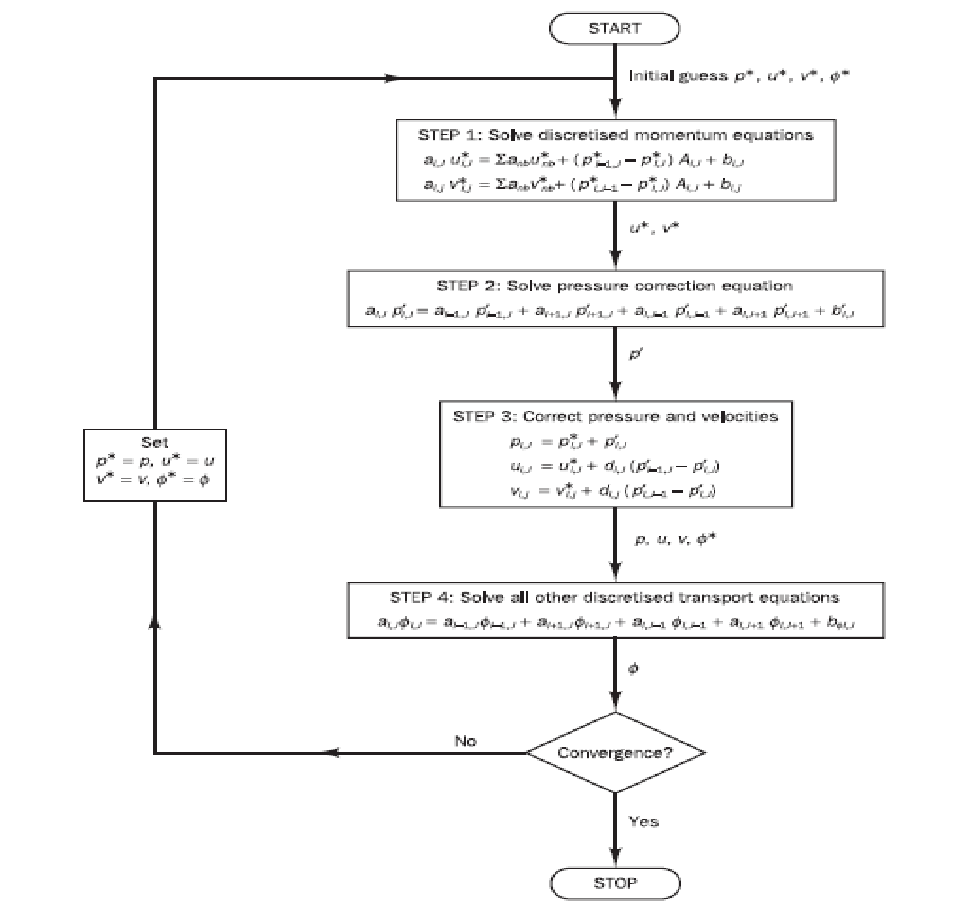
\includegraphics[width=0.7\linewidth]{12.nal_slike/SIMPLE.png}
    \caption{Blokovni diagram SIMPLE algoritma}
\end{figure}

\subsubsection{Algoritem PISO}

PISO (pressure implicit with splitting of operators) uporablja enake korake kot SIMPLE za 1. popravek, potem pa izvede še drugega
\begin{align}
    p^{***} &= p^{***} + p^{''}\\
    v^{***} &= v^{***} + v^{''}\nonumber
\end{align}
pri čemer se uporabi tudi izvendiagonalni del $O$ pri izračunu obeh popravkov.
\begin{align}
    &D\;L^{-1}\;G\;\mathbf{p^{''}} = -D\;O\;\mathbf{v^{'}}\\
    &\mathbf{v}^{''} = L^{-1}\;(-G\;\mathbf{p^{''}} -  O\;\mathbf{v^{'}})\nonumber
\end{align}

\begin{figure}[ht]
    \centering
    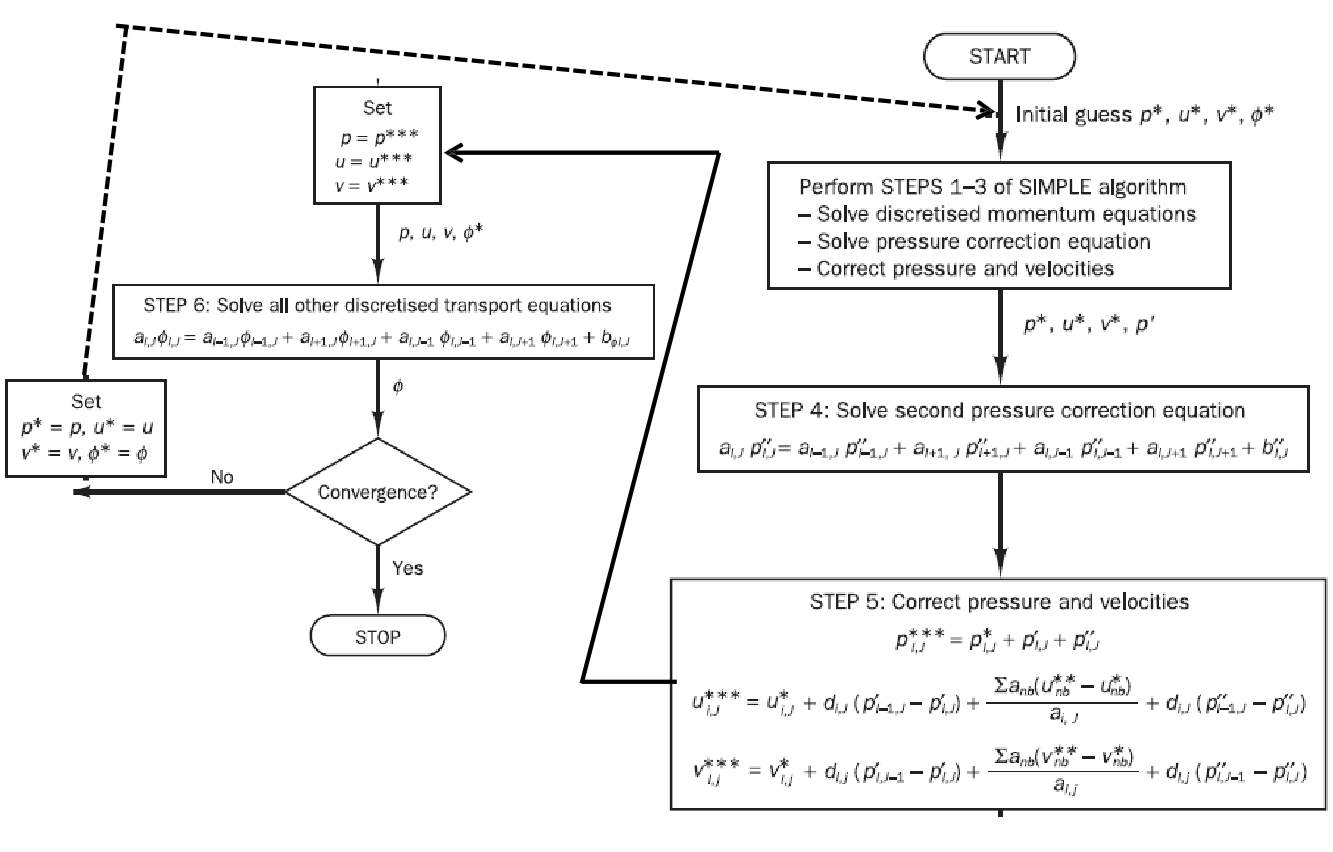
\includegraphics[width=0.8\linewidth]{12.nal_slike/PISO.png}
    \caption{Blokovni diagram PISO algoritma}
\end{figure}

\subsection{Numerični model}

Obravnavana domena je kvadrat s stranico dolžine 1. Na vseh, razen na zgornji strani, je hitrost enaka nič. Zgoraj pa je strižna komponenta hitrosti, torej v x-smeri enaka ena.

Za začetni približek tlačnega polja sem uporabil tlak povsod enak nič. Z boljšim približkom bi sicer lahko izboljšal konvergenco, vendar je tako enaka tudi začetna poskusna hitrost, kar olajša primejavo med reztultati. Uporabil sem zamaknjeno mrežo, kjer sem tlak računal v središčih KV, hitrosti pa na mejnih ploskvah. Na koncu sem za prikaz interpoliral hitrosti v središča KV.

Delujočega PISO algoritma mi ni uspelo usposobiti, zato so vsi rezultati izračunani s SIMPLE!

Silo na stranice sem izračunal iz zveze $d F_n = -p\; d A$, od koder sledi integral za silo na zgornji stranici, ki sem ga izračunal po Simpsonovi metodi
\begin{equation}
    F_y = -b\,\int_{0}^{1}\,p\,d x,
\end{equation}
kjer je $b=1$ širina kotanje. Izračunam pa lahko tudi sile na preostale robove kotanje.

\section{Hitrostno in tlačno polje}

Na spodnjih slikah je prikazan rezultat reševanja Navier-Stokesovih enačb - hitrostno in tlačno polje. Tekom iteracij simulacije sem spremljal potek obeh polj, residuale in hitrostni profil preko kotanje, ki je todi označen na levem grafu. Željena masna neuravnoteženost pod 0,01 je bila dosežena le pri nizkih $Re$ in manjšim število KV, saj drugače rešitev konvergira počasneje, da je rezultat stabilen, pa sem moral upoštevati pod-relaksacijske faktorje. Masna neuravnoteženost pomeni izpolnjevanje kontinuitne enačbe v diskretni obliki in sem jo računal tako, da sem seštel masno bilanco za vsak KV posebej.

Opazil sem tudi, da se z večanjem $Re$ večajo tudi stranski (protitočni) vrtinci, hitrostno polje postaja bolj nesimetrično, prav tako pa se spreminja lega središča glavnega vrtinca.

Opazil sem, da izbira diskretizacijske sheme ne vpliva močno na konvergenco, temveč predvsem na rezultat, sploh pri večjih hitrostih, saj centralna diferenčna shema ni primerna za Pecletova števila $Pe=\frac{\rho\;u\;h}{D}$ večja od 2, zato sem pri uprabih hibridno shemo, ki za $Pe<2$ upošteva centralno, drugače pa privetrno shemo.

\begin{figure}[H]
    \centering
    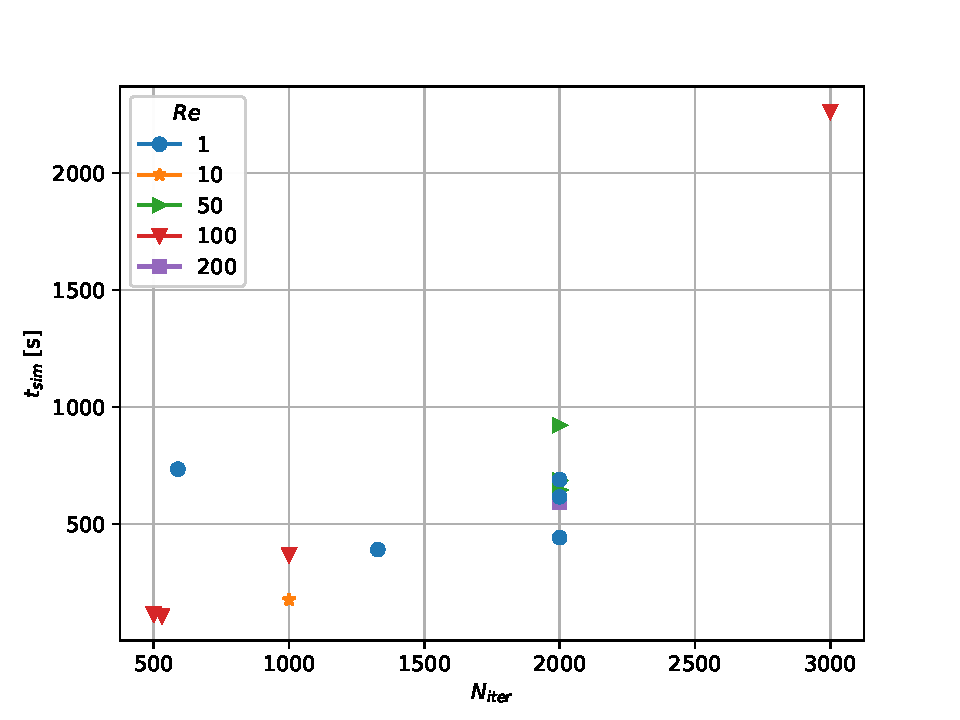
\includegraphics[width=0.6\linewidth]{12.nal_slike/t_sim.pdf}
    \caption{Časovna zahtevnost simulacij}
\end{figure}

\begin{figure}[H]
    \centering
    \begin{subfigure}{0.49\textwidth}
        \centering
        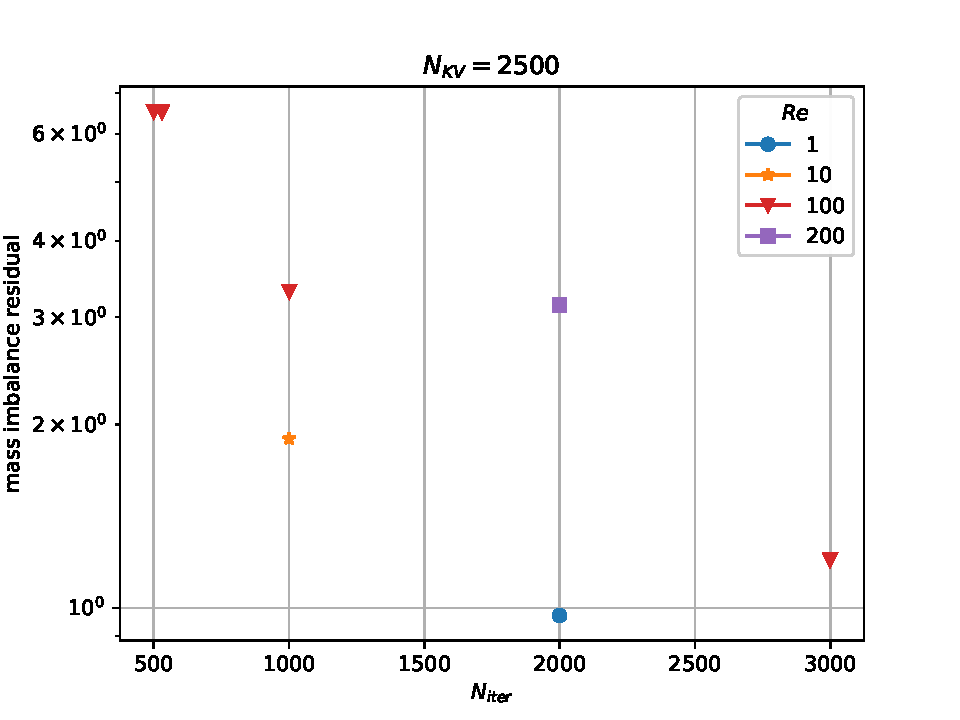
\includegraphics[width=\linewidth]{12.nal_slike/imbalance_Niter.pdf}
        \caption{pri $N_{KV}=2500$}        
    \end{subfigure}
    \begin{subfigure}{0.49\textwidth}
        \centering
        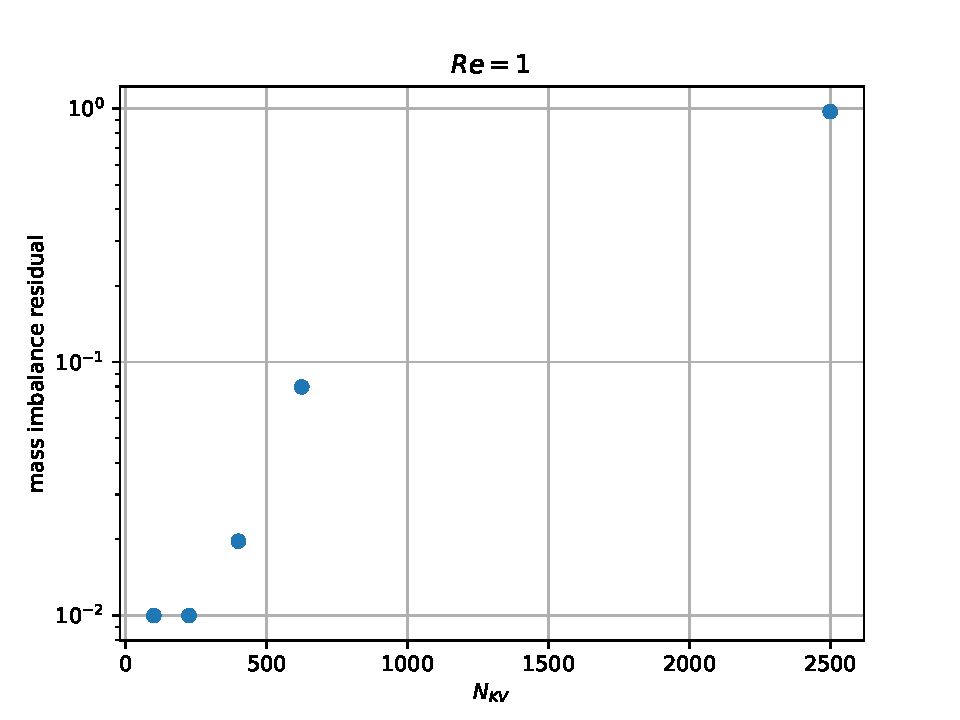
\includegraphics[width=\linewidth]{12.nal_slike/imbalance_Nkv.pdf}
        \caption{pri $Re=1$ do željene izboljšave 0,01}        
    \end{subfigure}
    \caption{Masna neuravnoteženost}
\end{figure}

\subsection{Re = 1}

Hitrostni profil je simetričen, pod-relaksacija ni bila potrebna.

\begin{figure}[H]
    \centering
    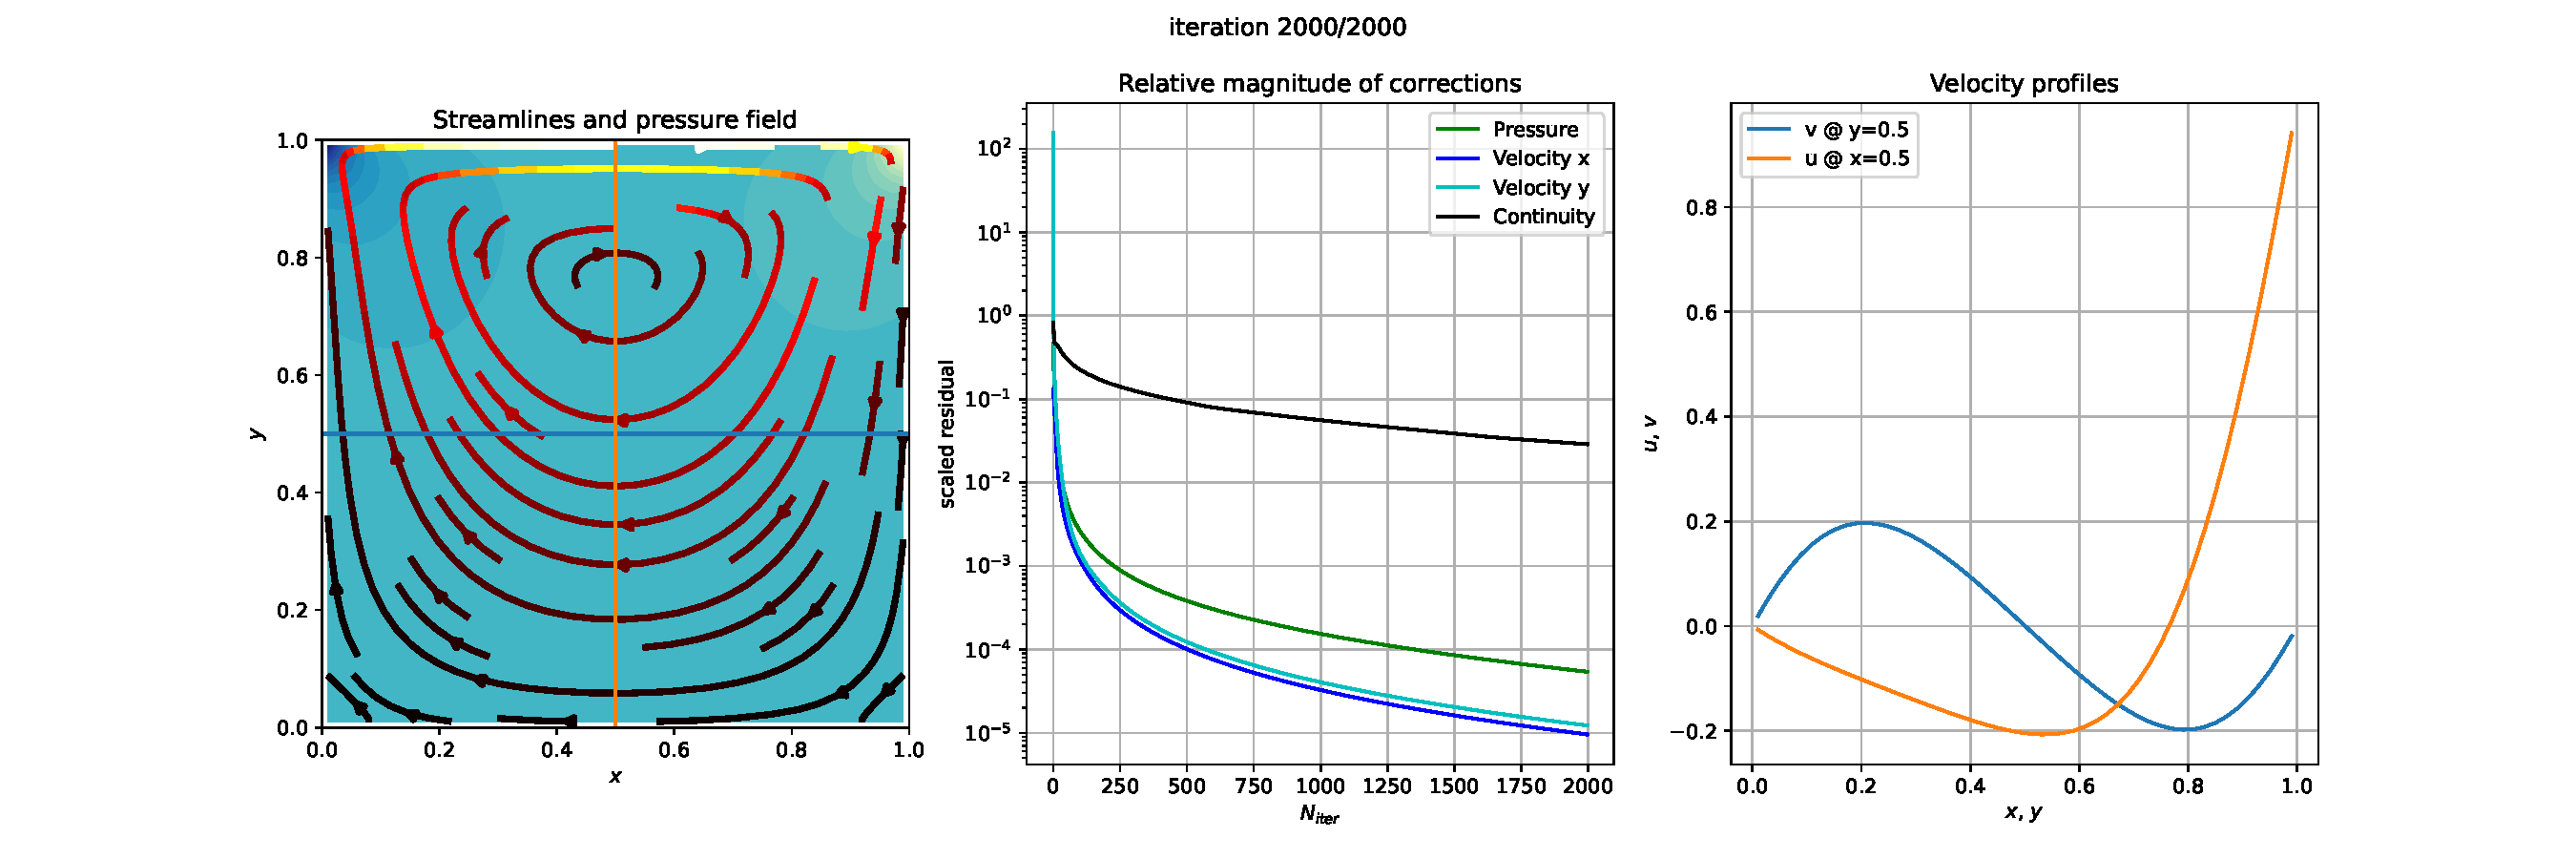
\includegraphics[width=\linewidth]{12.nal_slike/Re1.pdf}
    \caption{Konvergenca pri $Re=1$}
\end{figure}

\begin{figure}[H]
    \centering
    \begin{subfigure}{0.49\textwidth}
        \centering
        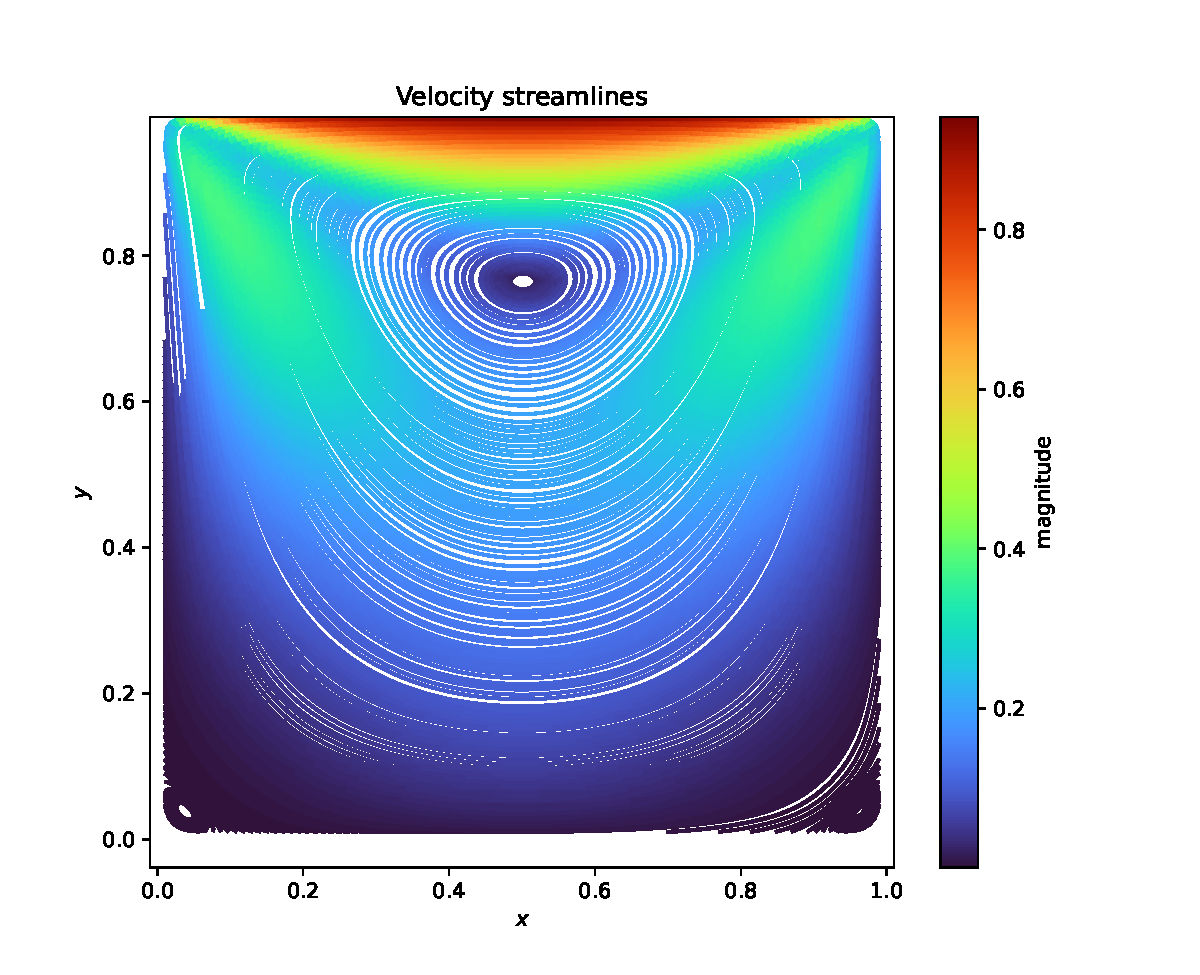
\includegraphics[width=\linewidth]{12.nal_slike/Re1_tok.pdf}
        \caption{tokovnice}
    \end{subfigure}
    \begin{subfigure}{0.49\textwidth}
        \centering
        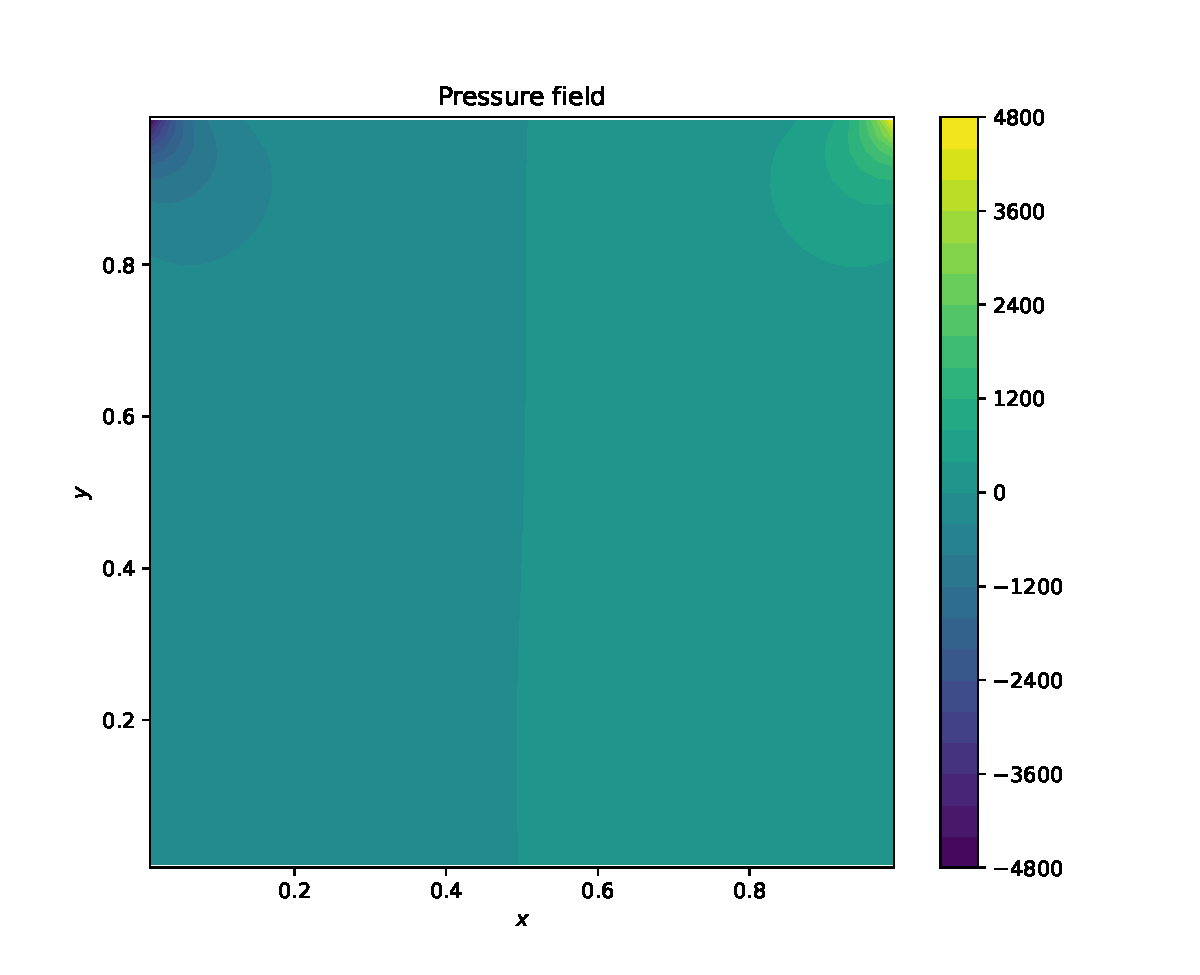
\includegraphics[width=\linewidth]{12.nal_slike/Re1_p.pdf}
        \caption{tlačno polje}
    \end{subfigure}
    \caption{Rezultati za $Re=1$}
\end{figure}

\subsection{Re = 10}

Tudi pri $Re=10$ pod-relaksacija še ni potrebna, vrtinci v robovih so že bolj izraziti.

\begin{figure}[H]
    \centering
    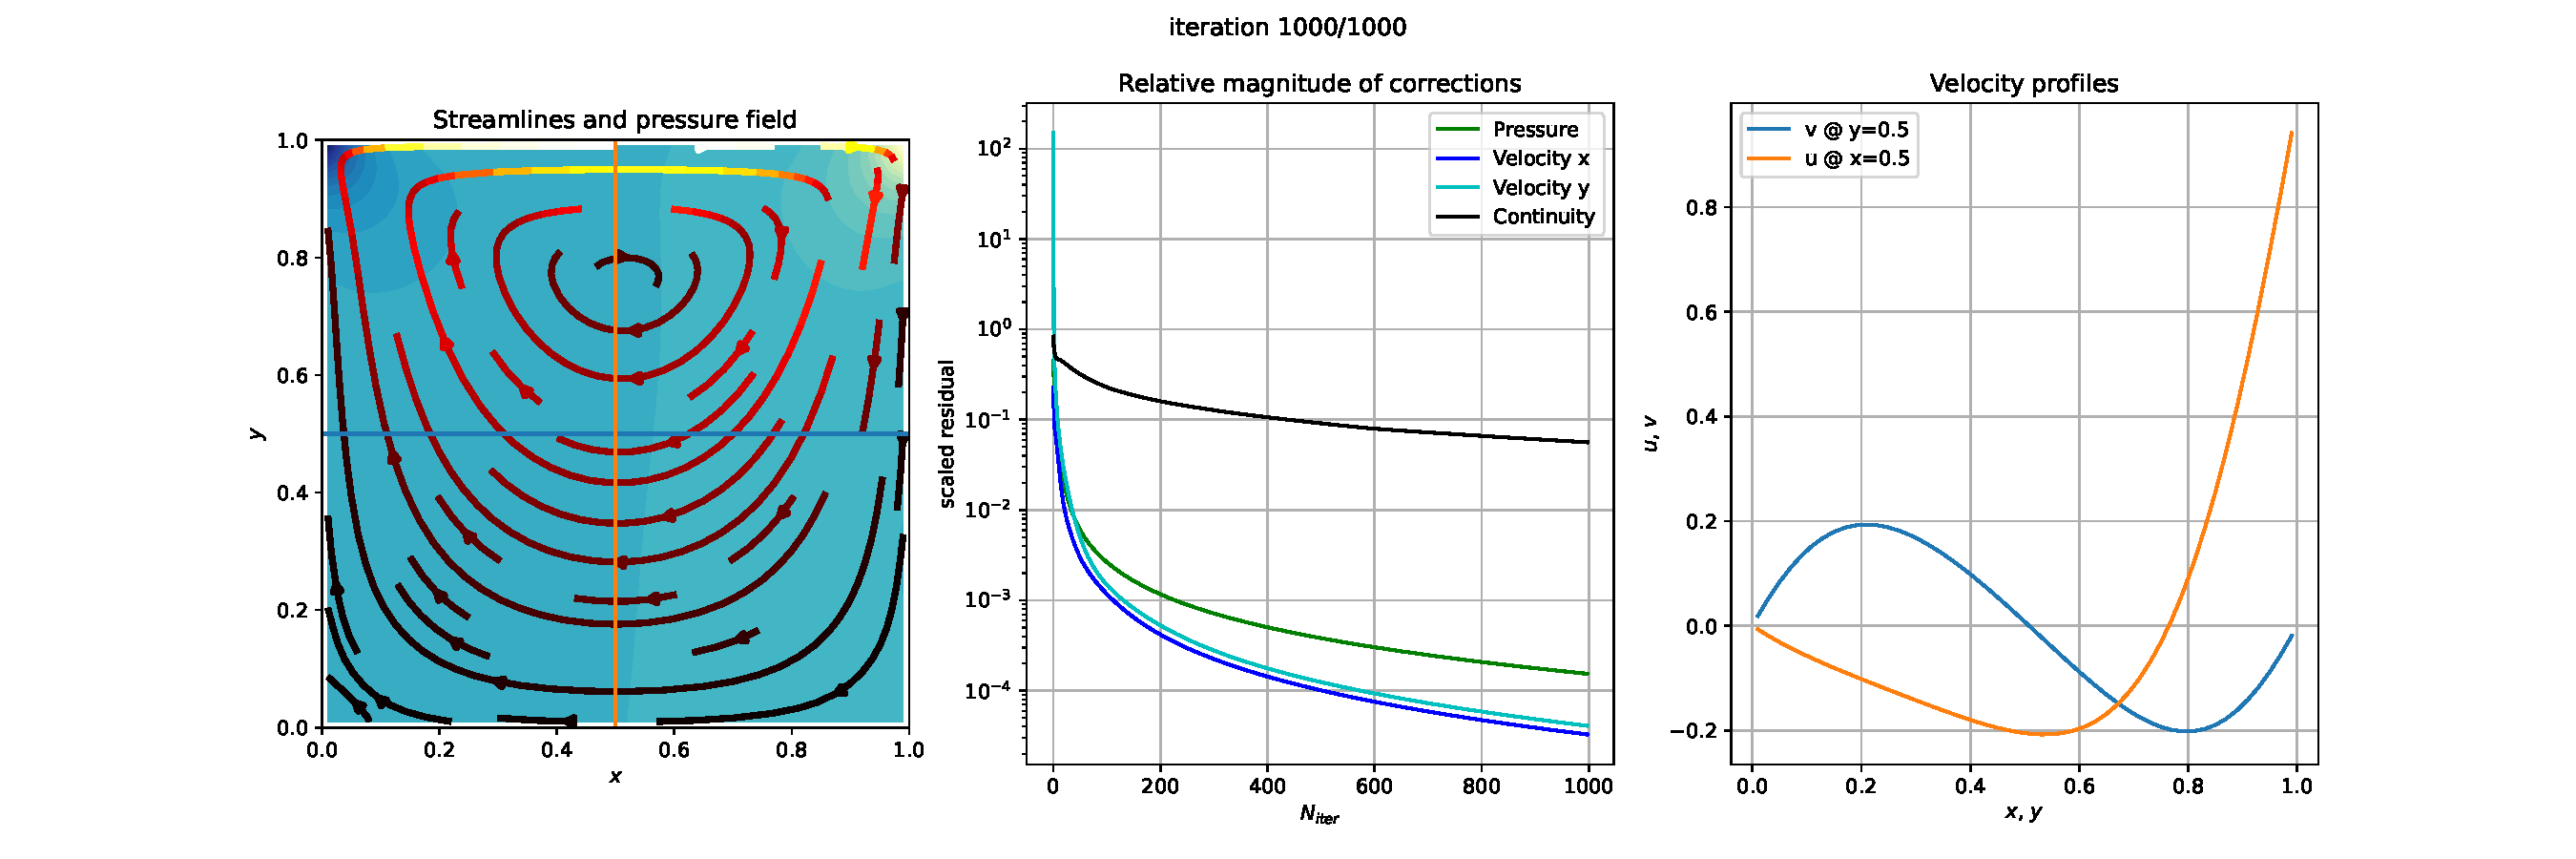
\includegraphics[width=\linewidth]{12.nal_slike/Re10.pdf}
    \caption{Konvergenca pri $Re=10$}
\end{figure}

\begin{figure}[H]
    \centering
    \begin{subfigure}{0.49\textwidth}
        \centering
        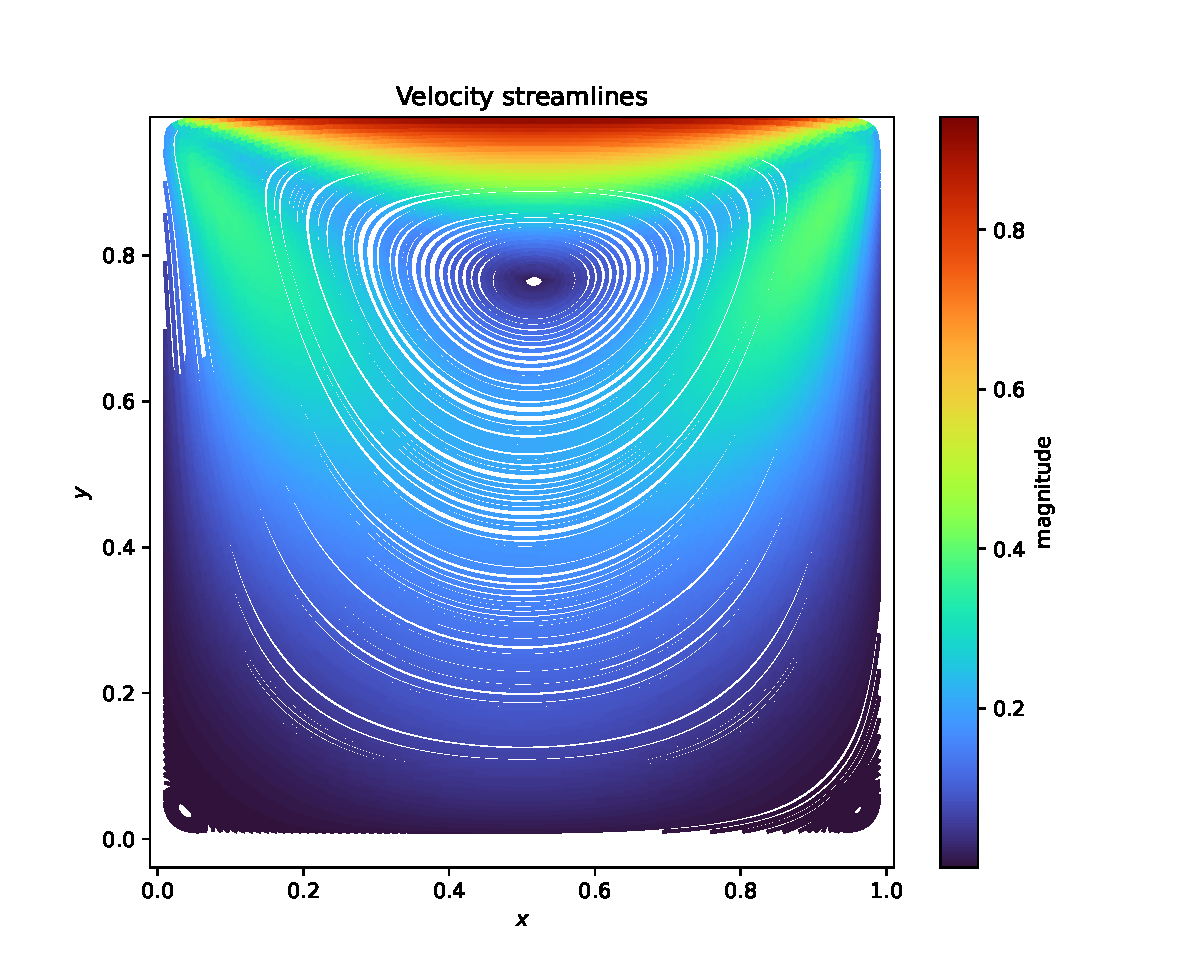
\includegraphics[width=\linewidth]{12.nal_slike/Re10_tok.pdf}
        \caption{tokovnice}
    \end{subfigure}
    % \begin{subfigure}{0.49\textwidth}
    %     \centering
    %     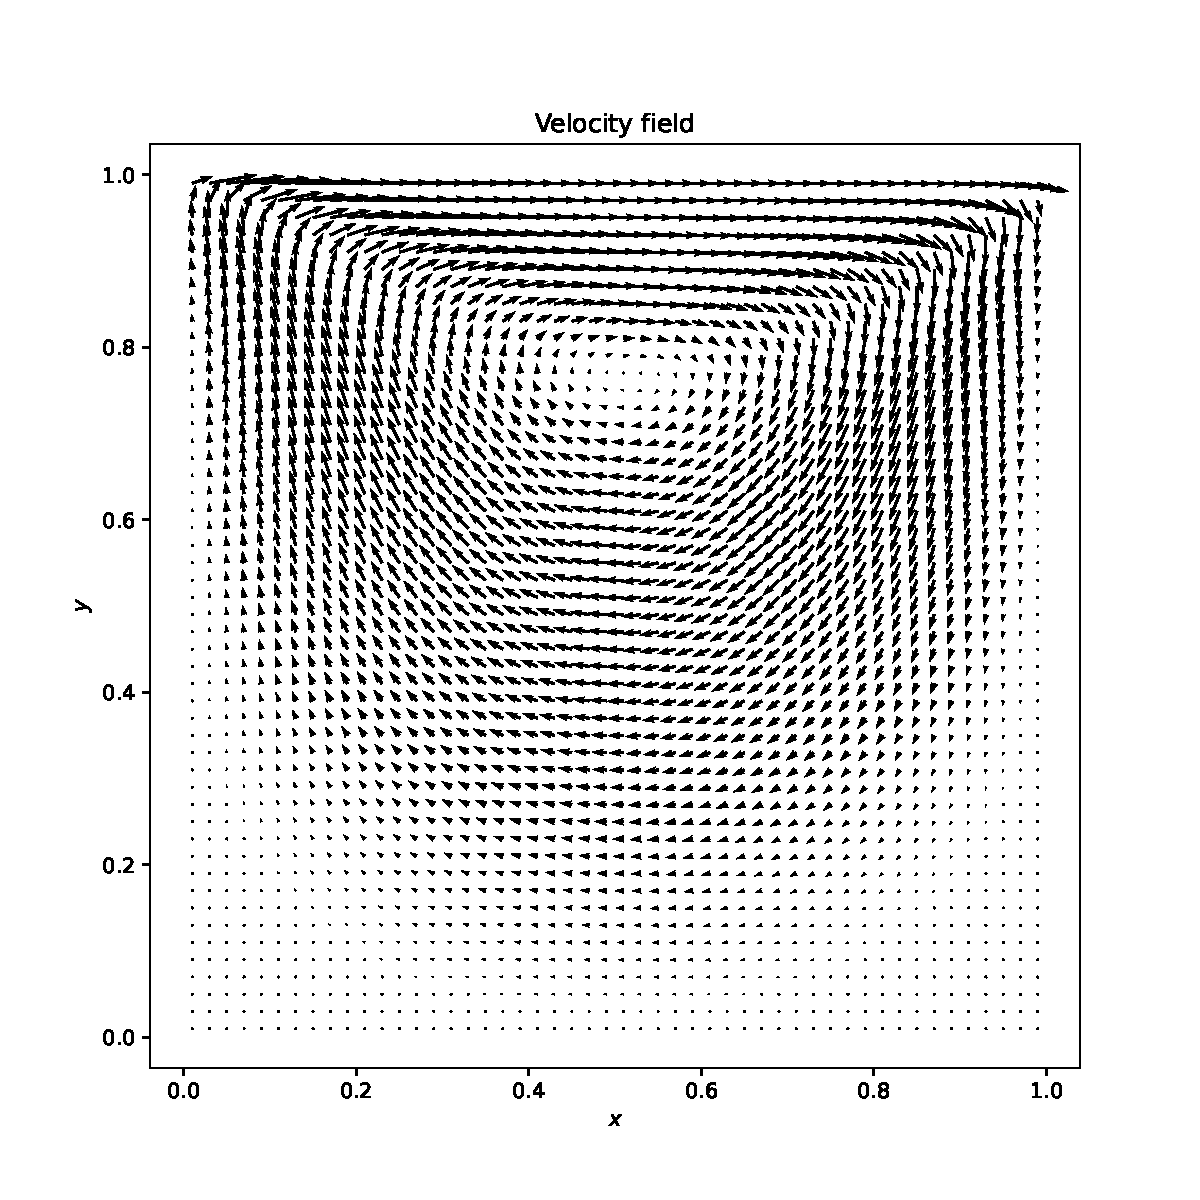
\includegraphics[width=\linewidth]{12.nal_slike/Re10_vec.pdf}
    %     \caption{hitrostno polje}
    % \end{subfigure}
    \begin{subfigure}{0.49\textwidth}
        \centering
        \includegraphics[width=\linewidth]{12.nal_slike/Re10_p.pdf}
        \caption{tlačno polje}
    \end{subfigure}
    \caption{Rezultati za $Re=10$}
\end{figure}

\subsection{Re = 50}

Hitrostni profil je že očitno nesimetričen, vendar rešitev konvergira tudi brez relaksacije.

\begin{figure}[H]
    \centering
    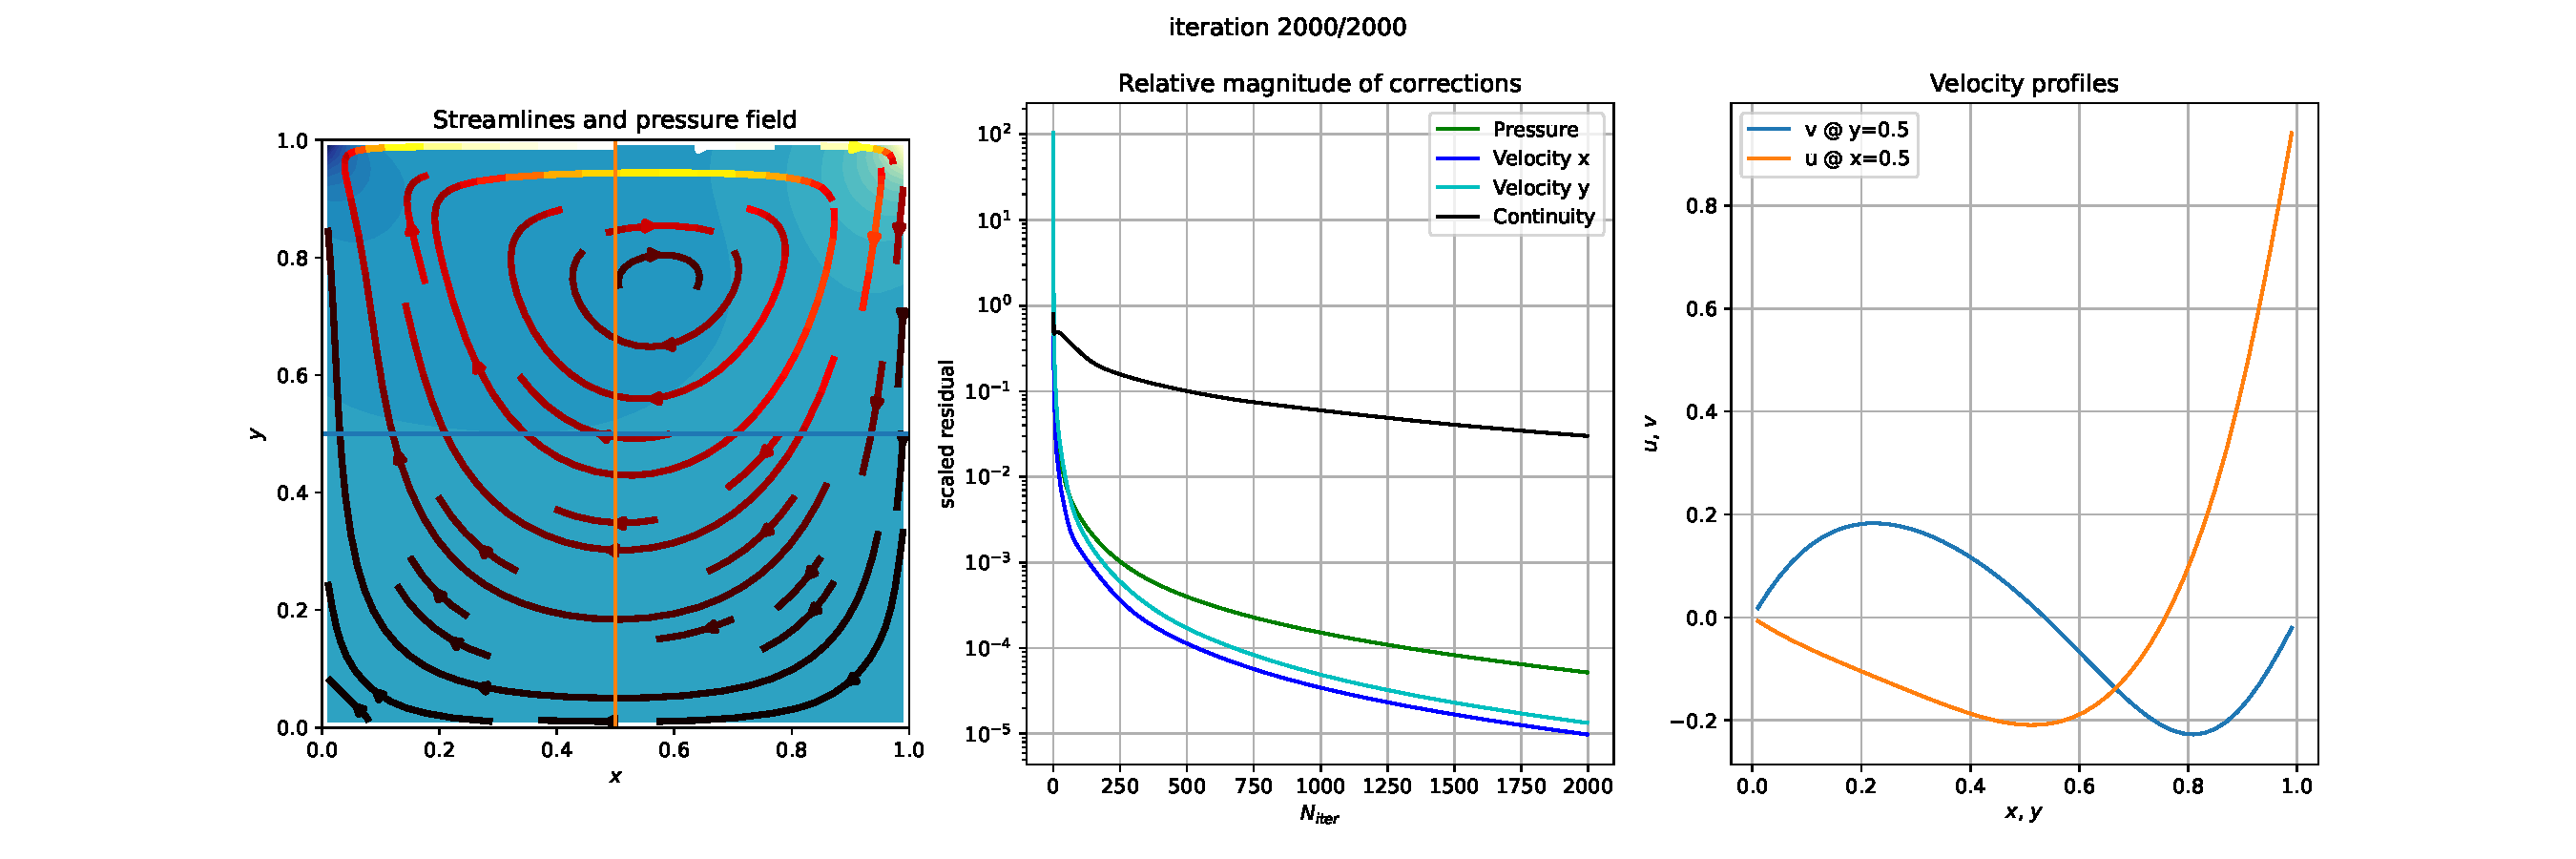
\includegraphics[width=\linewidth]{12.nal_slike/Re50.pdf}
    \caption{Konvergenca pri $Re=50$}
\end{figure}

\begin{figure}[H]
    \centering
    \begin{subfigure}{0.49\textwidth}
        \centering
        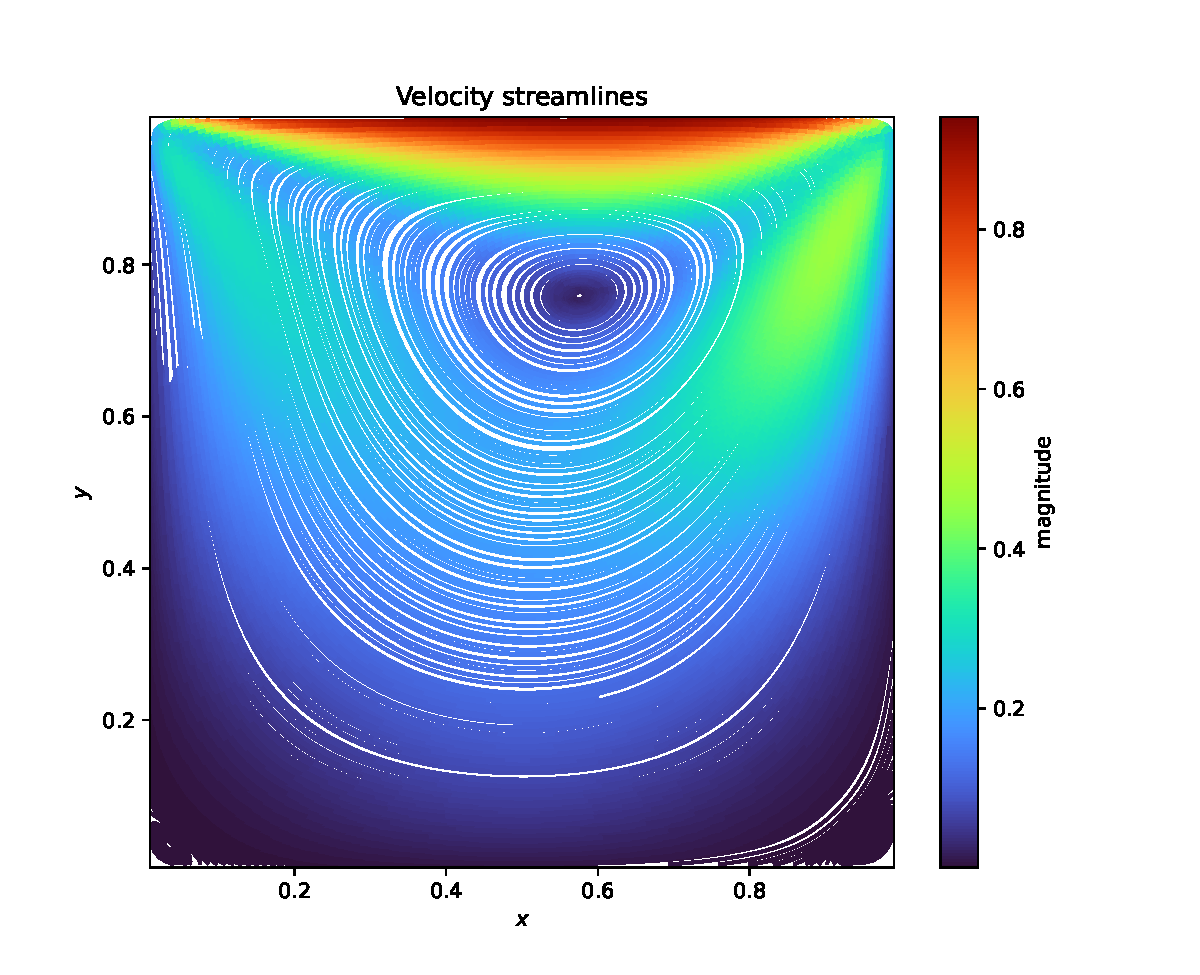
\includegraphics[width=\linewidth]{12.nal_slike/Re50_tok.pdf}
        \caption{tokovnice}
    \end{subfigure}
    \begin{subfigure}{0.49\textwidth}
        \centering
        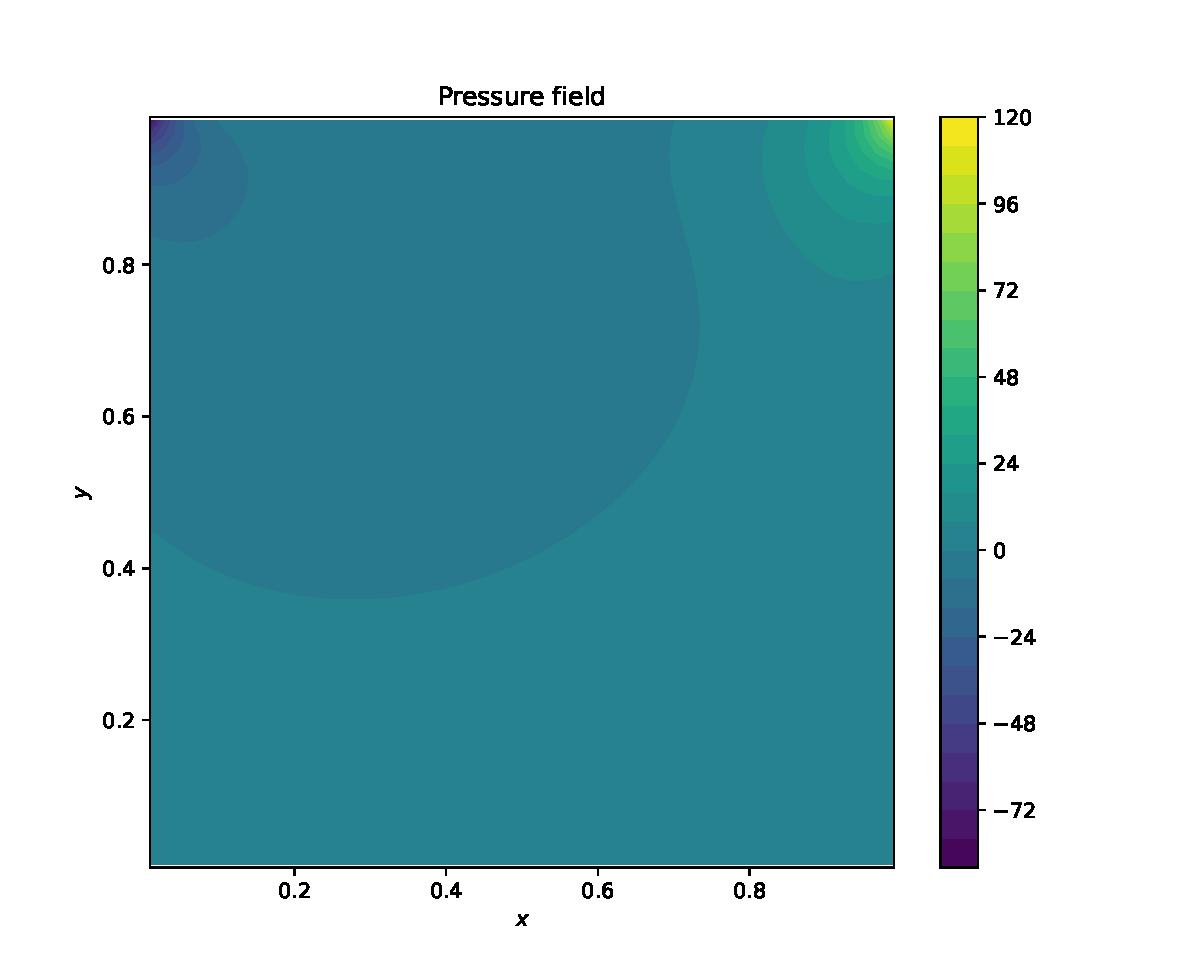
\includegraphics[width=\linewidth]{12.nal_slike/Re50_p.pdf}
        \caption{tlačno polje}
    \end{subfigure}
    \caption{Rezultati za $Re=50$}
\end{figure}

\subsection{Re = 100}

Tukaj sem uporabil relaksacijski koeficient za tlačni popravek 0,7 in za hitrost 0,5, saj je drugače rešitev pri okoli 500 iteracijah začela divergirati. Na to ni pretirano vplivala diskretizacijska shema, prav tako pa tudi ne na rezultate.

\begin{figure}[H]
    \centering
    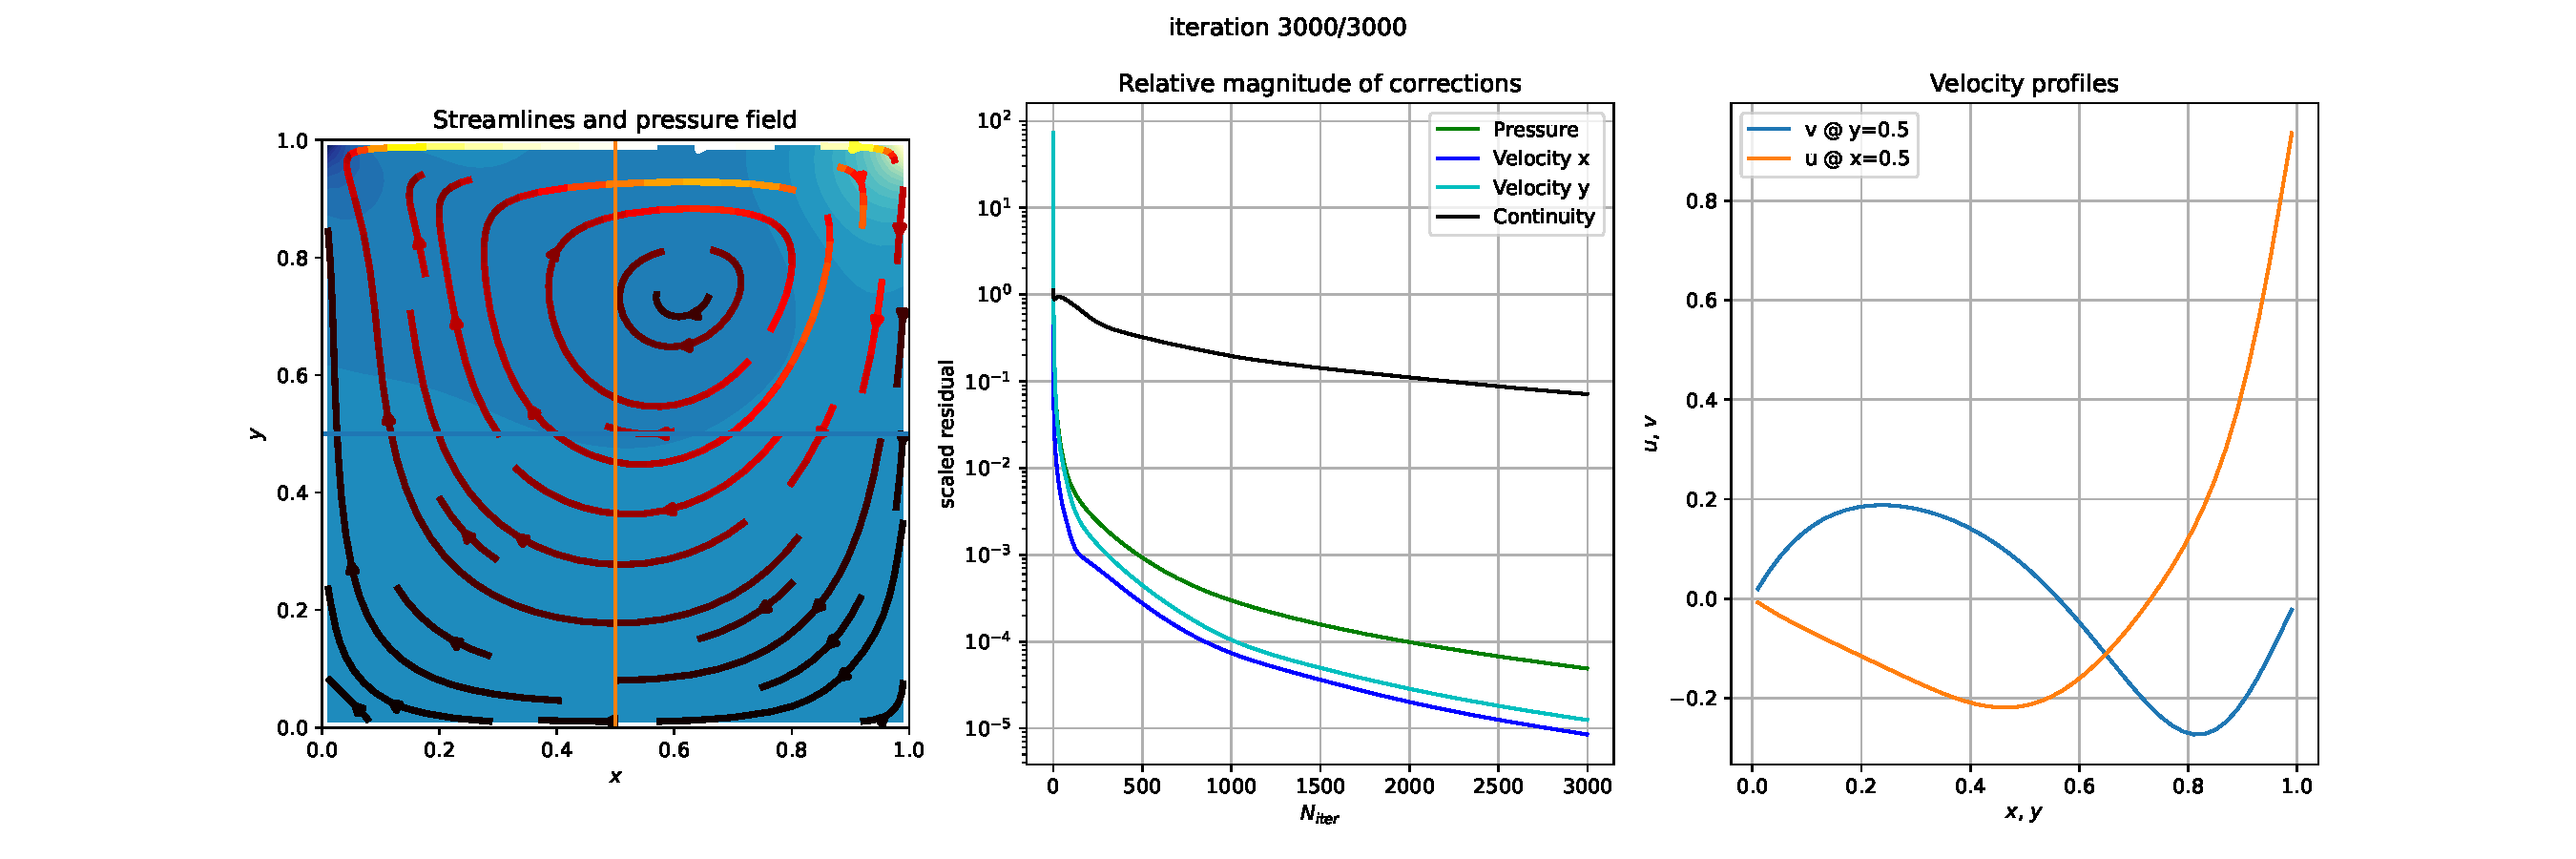
\includegraphics[width=\linewidth]{12.nal_slike/Re100.pdf}
    \caption{Konvergenca pri $Re=100$}
\end{figure}

\begin{figure}[H]
    \centering
    \begin{subfigure}{0.49\textwidth}
        \centering
        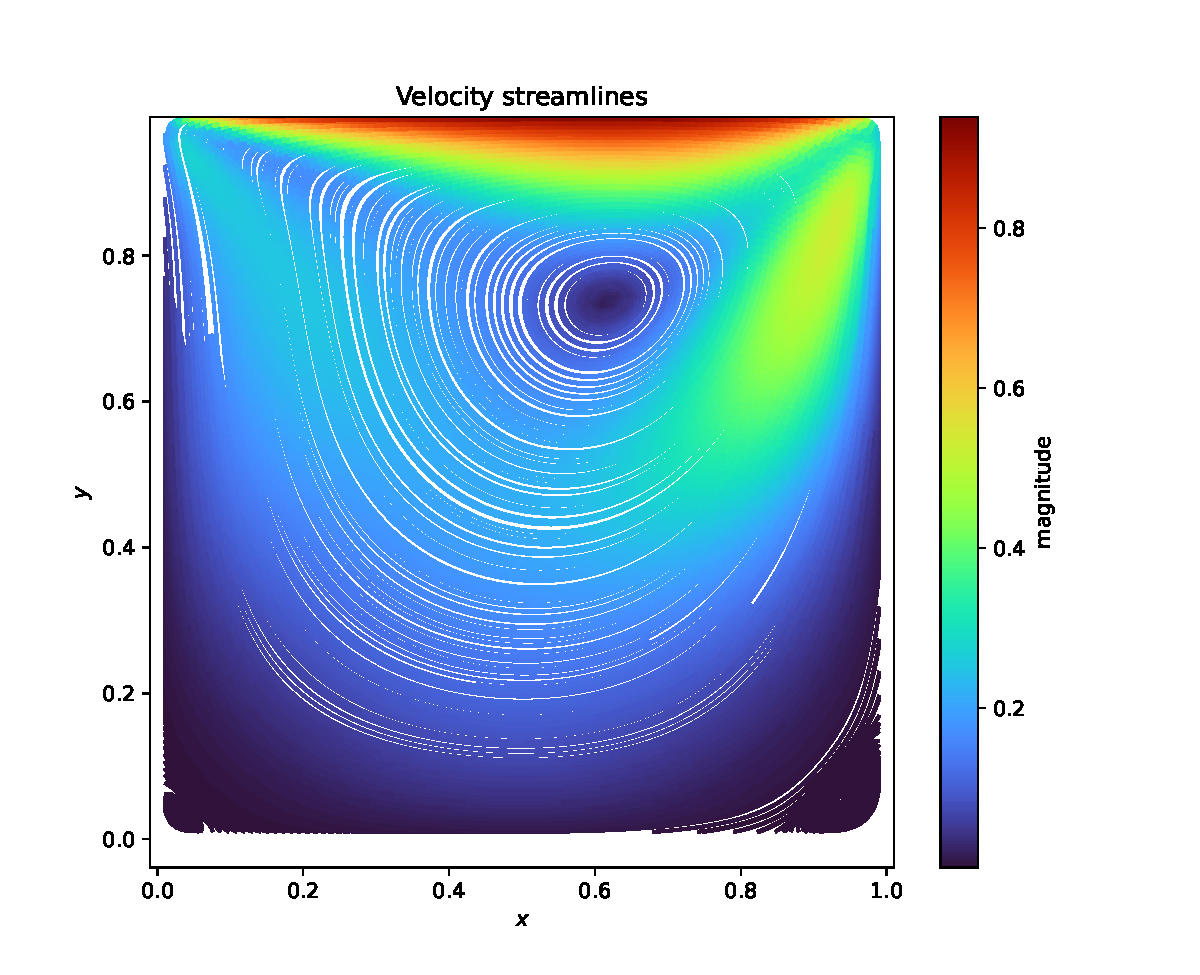
\includegraphics[width=\linewidth]{12.nal_slike/Re100_tok.pdf}
        \caption{tokovnice}
    \end{subfigure}
    \begin{subfigure}{0.49\textwidth}
        \centering
        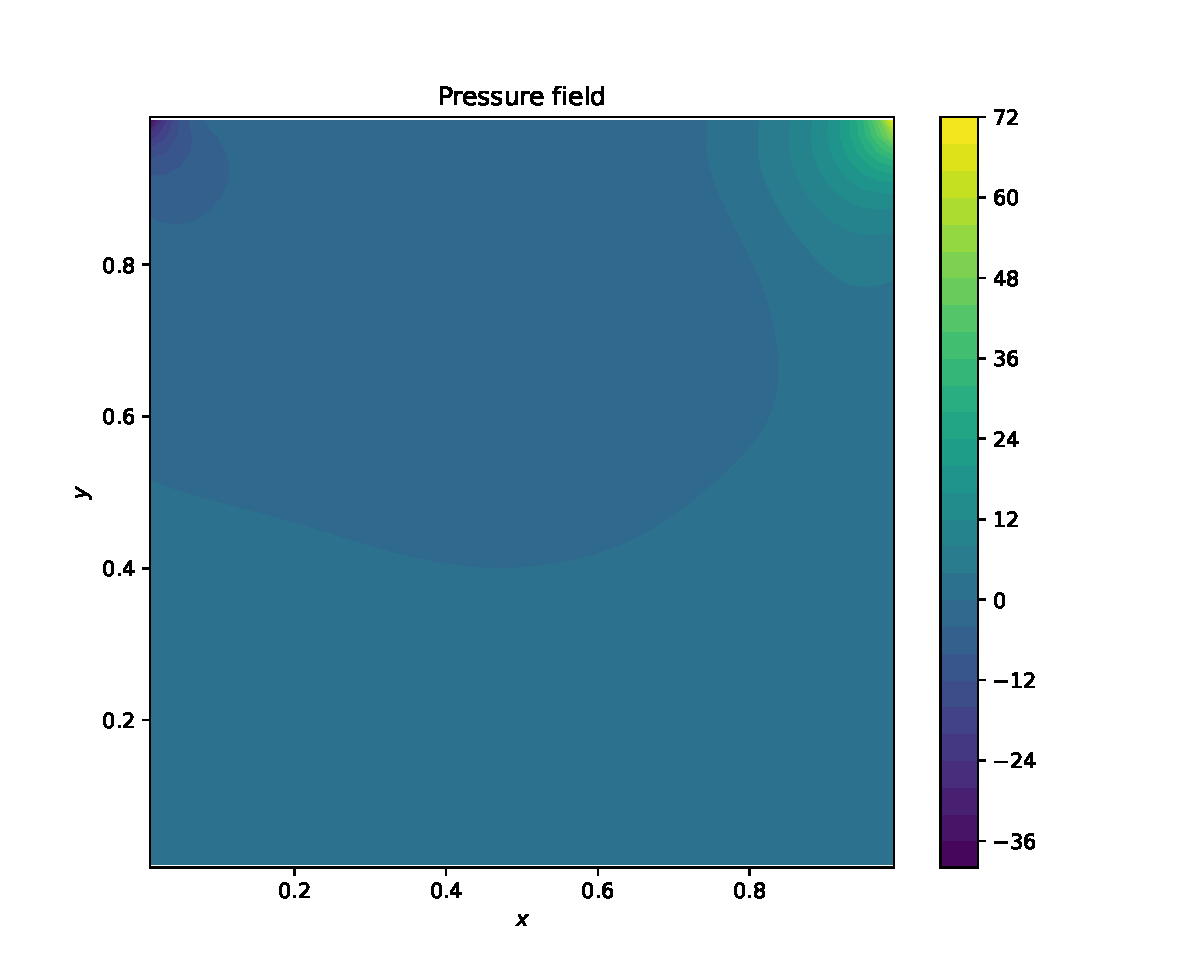
\includegraphics[width=\linewidth]{12.nal_slike/Re100_p.pdf}
        \caption{tlačno polje}
    \end{subfigure}
    \caption{Rezultati za $Re=100$}
\end{figure}

\subsection{Re = 200}

Relaksacijske koeficiente sem še dodatno zmanjšal, predvsem za hitrost na 0,2 in za tlak na 0,6. Pri večjih Re je potrebno tudi več iteracij za enako vrednost izboljšave masne neuravnoteženosti, da je ta še vedno pod $10^{-1}$.

\begin{figure}[H]
    \centering
    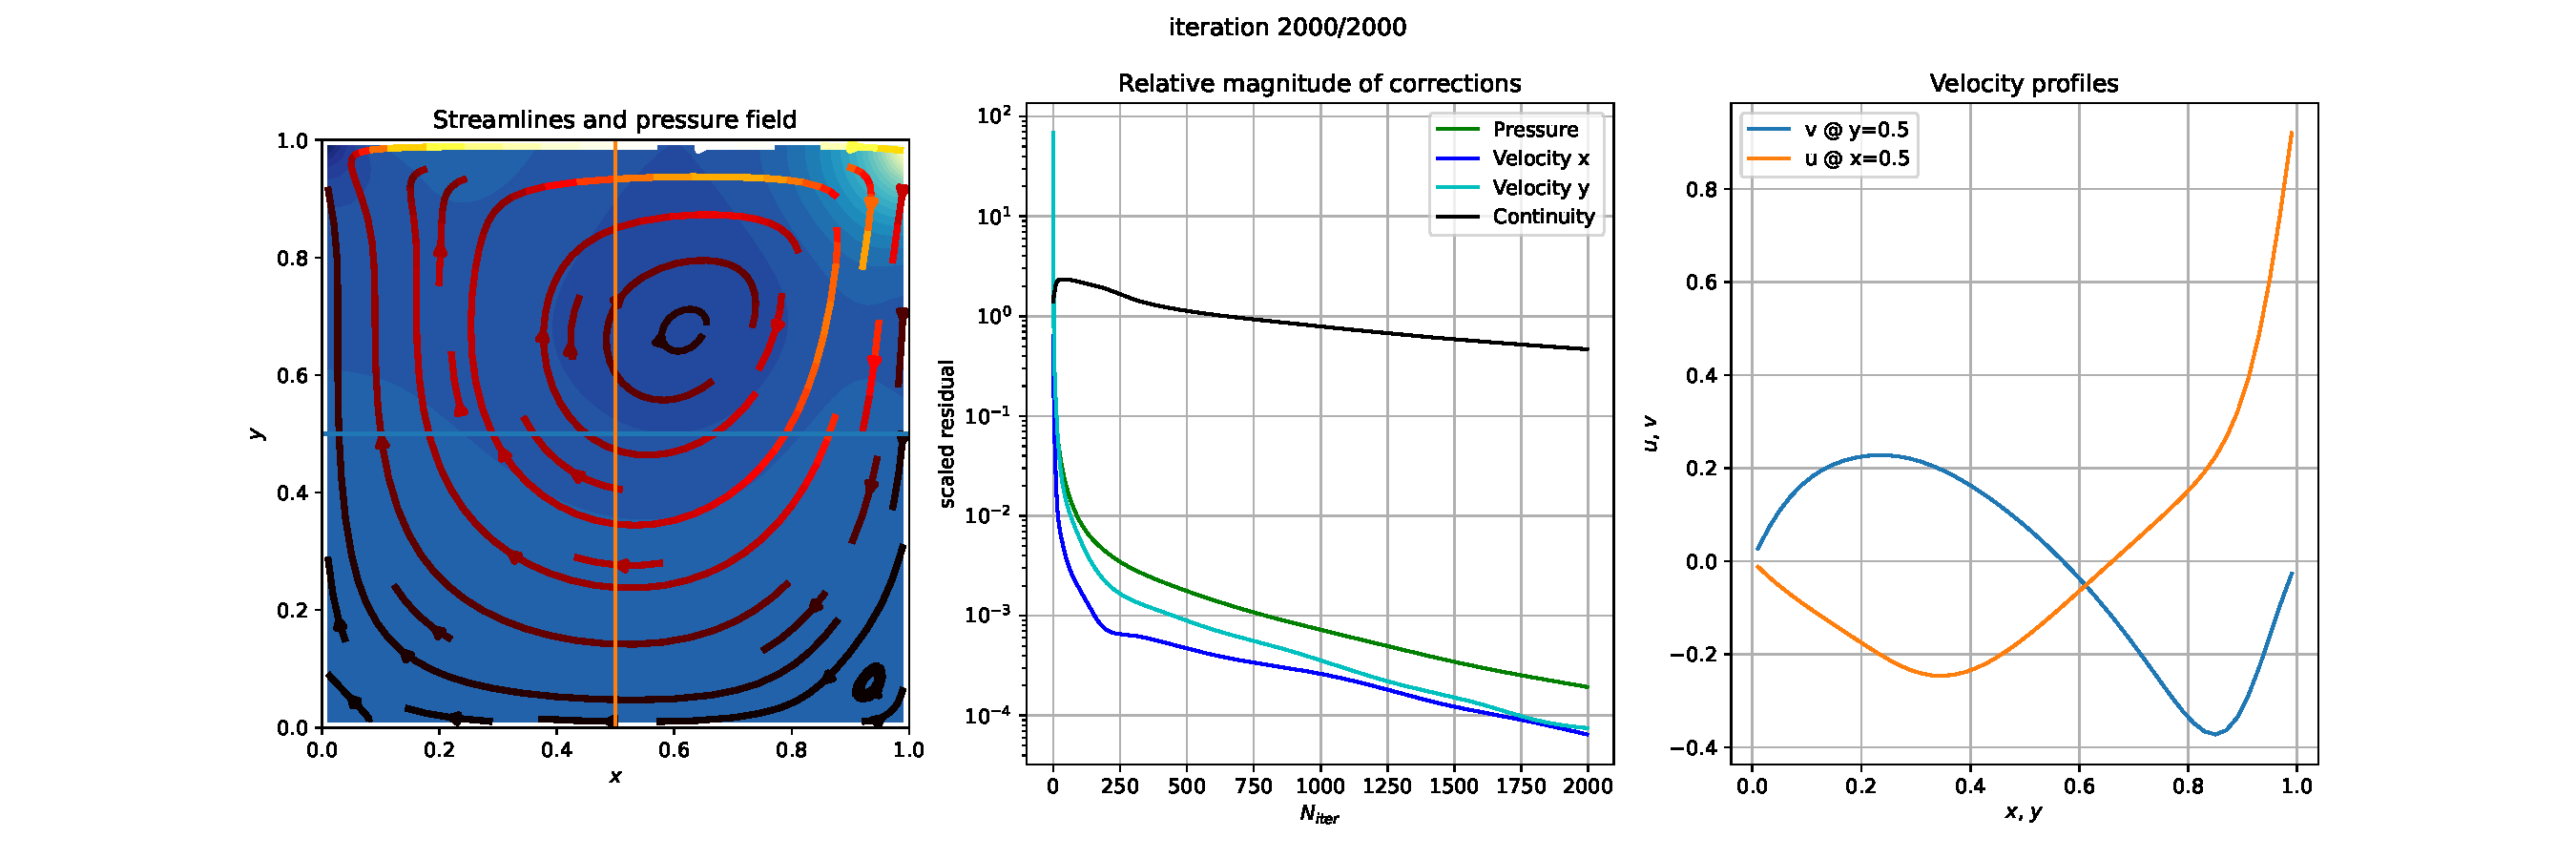
\includegraphics[width=\linewidth]{12.nal_slike/Re200.pdf}
    \caption{Konvergenca pri $Re=200$}
\end{figure}

\begin{figure}[H]
    \centering
    \begin{subfigure}{0.49\textwidth}
        \centering
        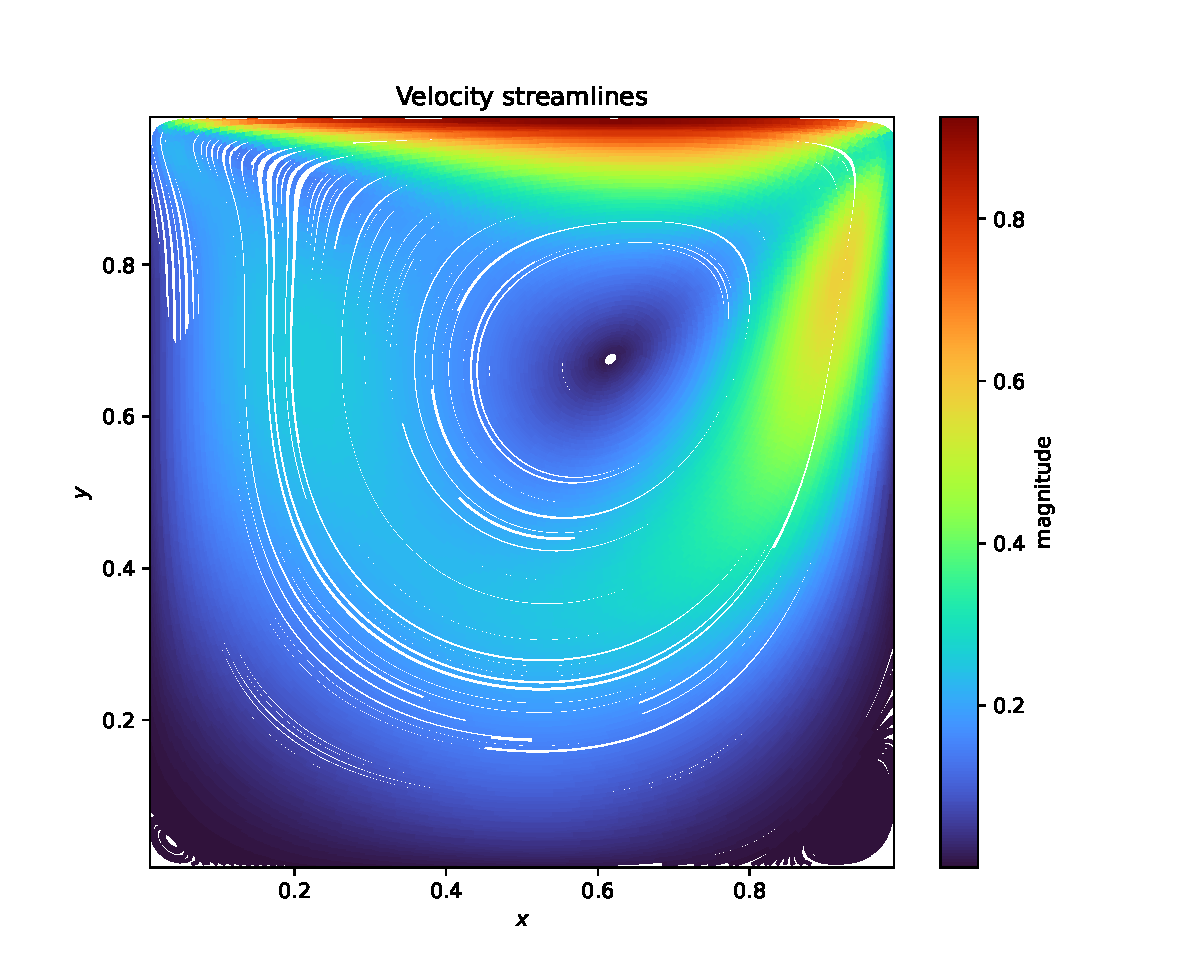
\includegraphics[width=\linewidth]{12.nal_slike/Re200_tok.pdf}
        \caption{tokovnice}
    \end{subfigure}
    \begin{subfigure}{0.49\textwidth}
        \centering
        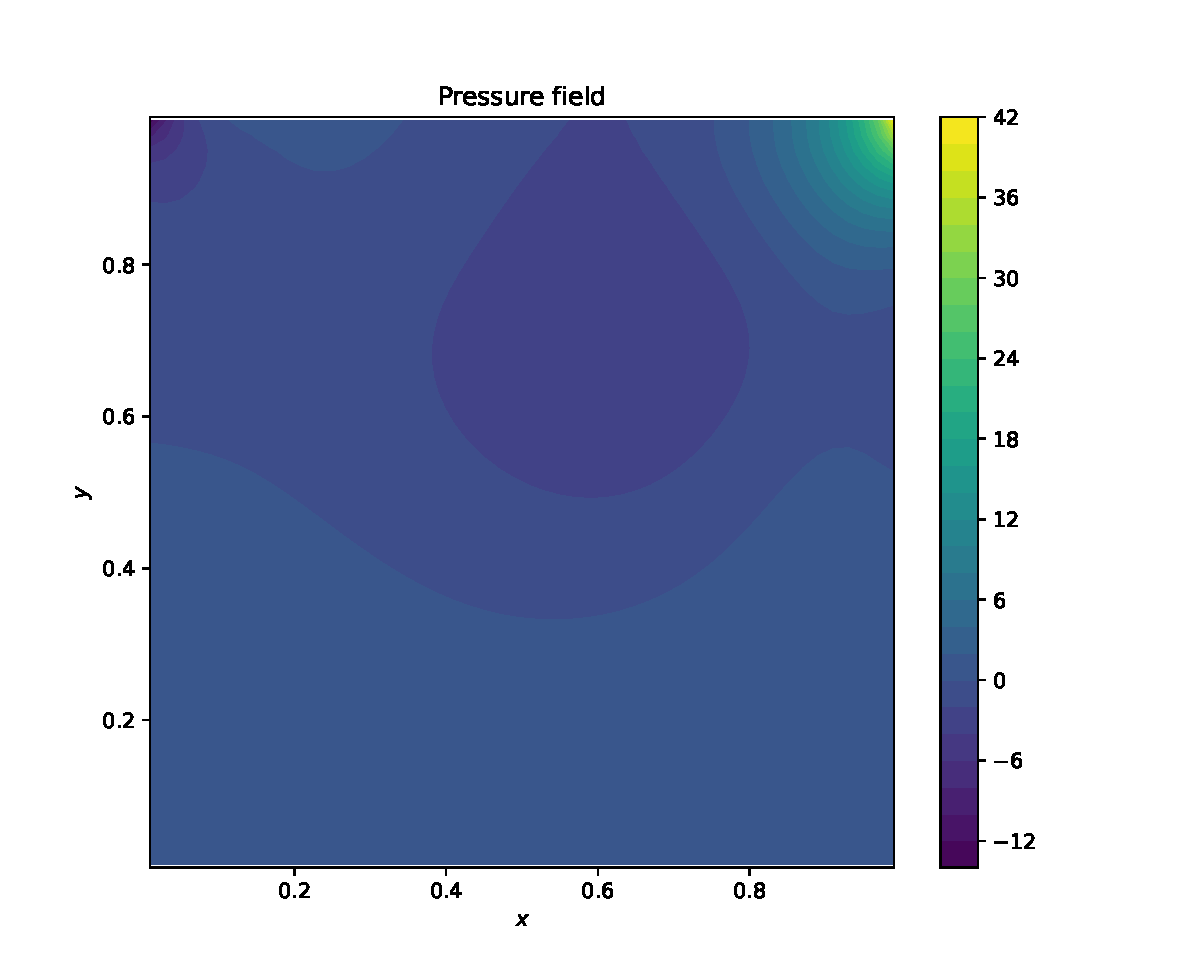
\includegraphics[width=\linewidth]{12.nal_slike/Re200_p.pdf}
        \caption{tlačno polje}
    \end{subfigure}
    \caption{Rezultati za $Re=200$}
\end{figure}

\subsection{Re = 800}

V tem primeru so bile velike težave s konvergenco; relaksacijske koeficiente sem zmanjšal na 0,3 za tlak in 0,1 za hitrost, saj je sicer rešitev podivjala, zato pa je bila konvergenca zelo počasna. Po zaključku 4000 iteracij je bila masna neuravnoteženost okoli 7, vseeno pa rezultati niso popolnoma nesmiselni.

\begin{figure}[ht]
    \centering
    \begin{subfigure}{0.49\textwidth}
        \centering
        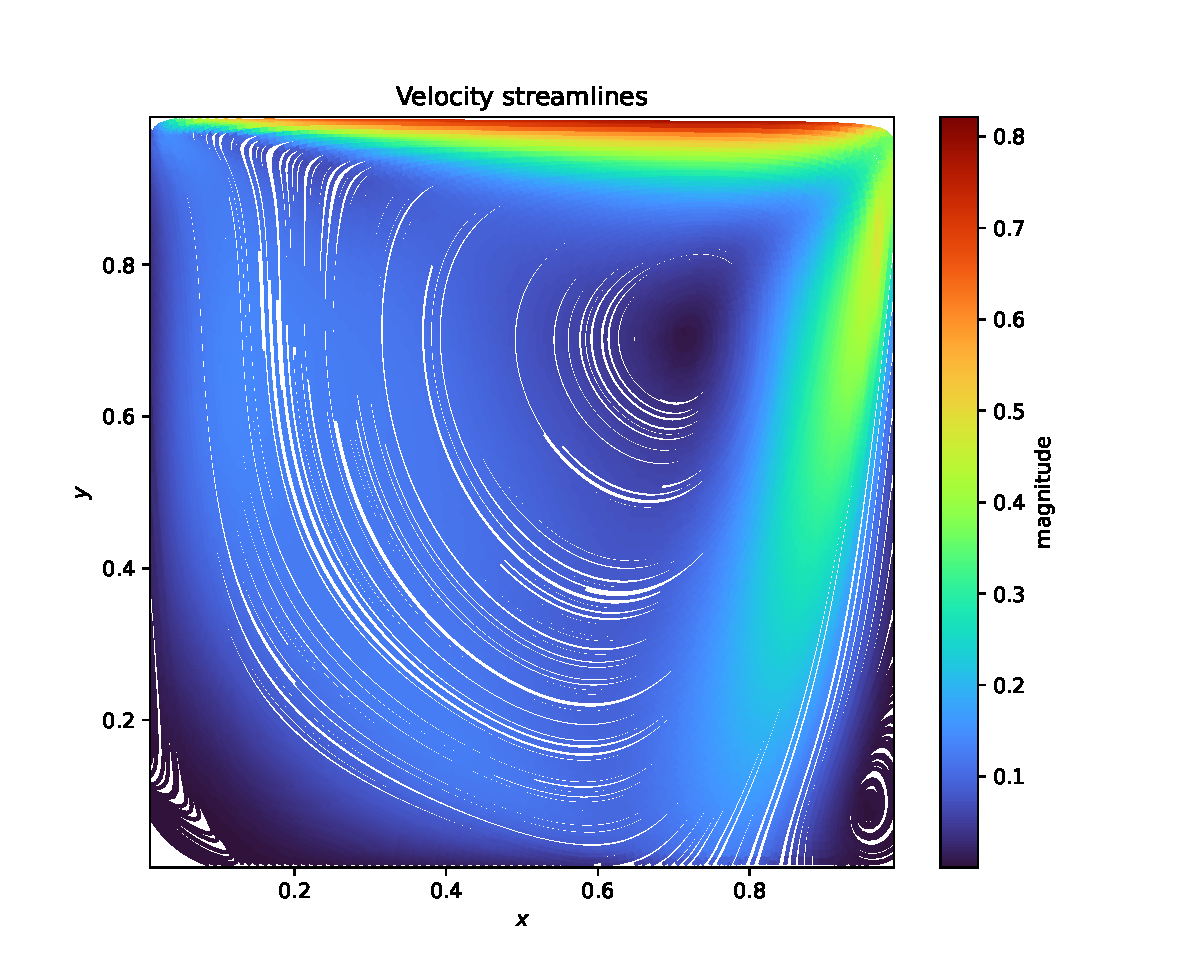
\includegraphics[width=\linewidth]{12.nal_slike/Re800_tok.pdf}
        \caption{tokovnice}
    \end{subfigure}
    \begin{subfigure}{0.49\textwidth}
        \centering
        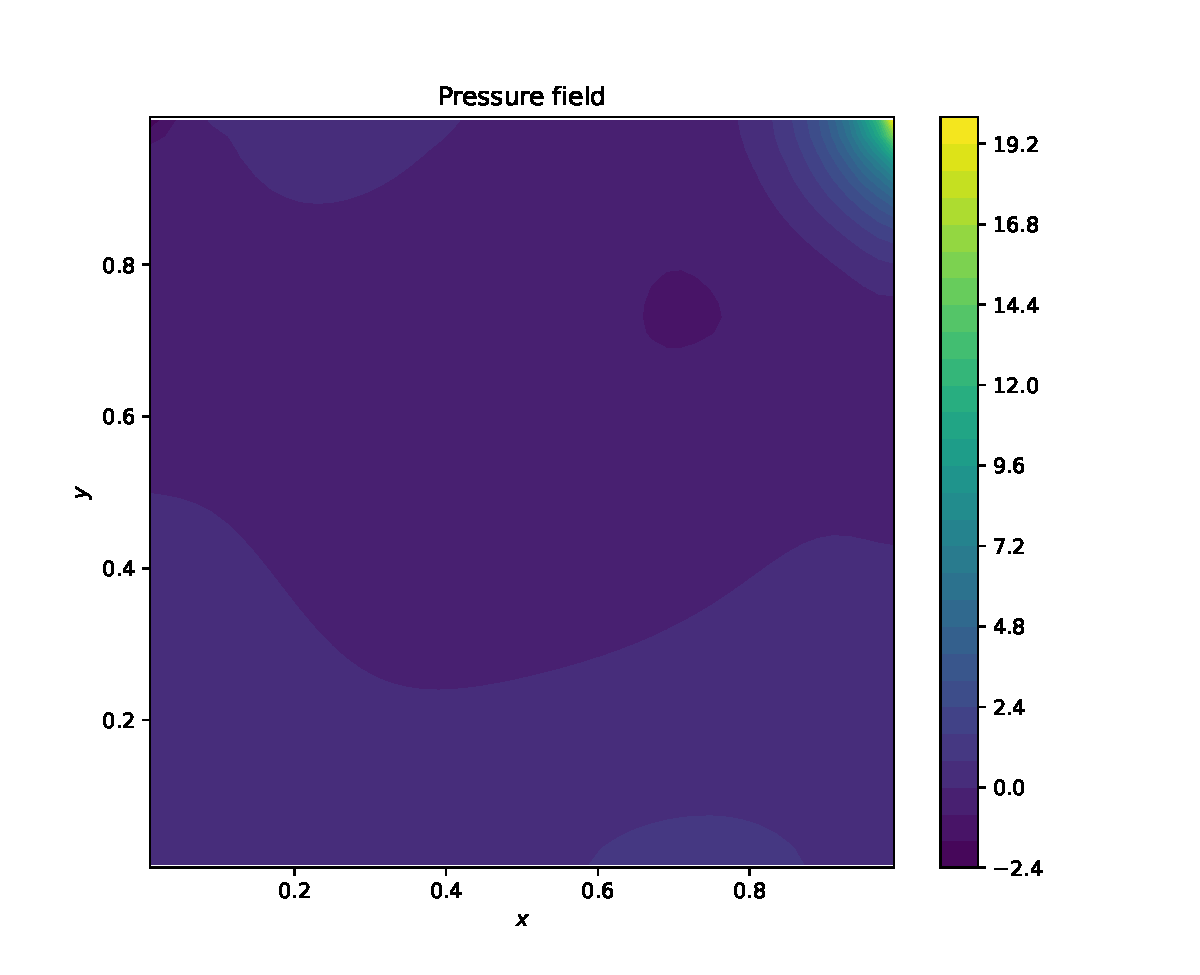
\includegraphics[width=\linewidth]{12.nal_slike/Re800_p.pdf}
        \caption{tlačno polje}
    \end{subfigure}
    \caption{Rezultati za $Re=800$}
\end{figure}


\begin{figure}[ht]
    \centering
    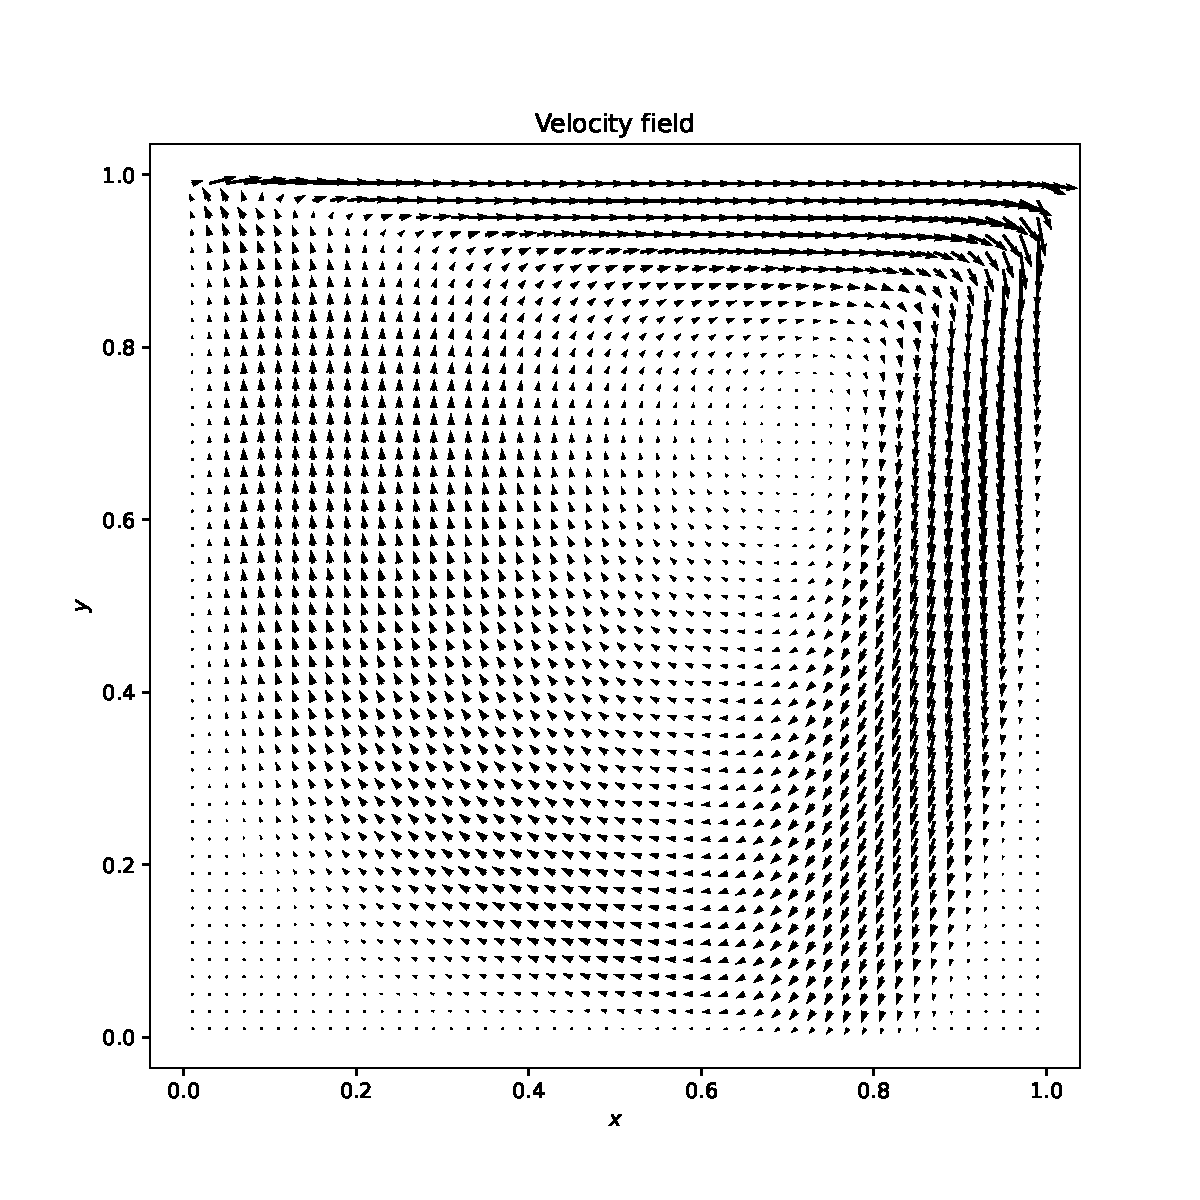
\includegraphics[width=\linewidth]{12.nal_slike/Re800_vec.pdf}
    \caption{Vektorsko polje hitrosti za $Re=800$}
\end{figure}

\section{Sile zaradi tlačnega polja}

\begin{figure}[H]
    \centering
    \begin{subfigure}{0.49\textwidth}
        \centering
        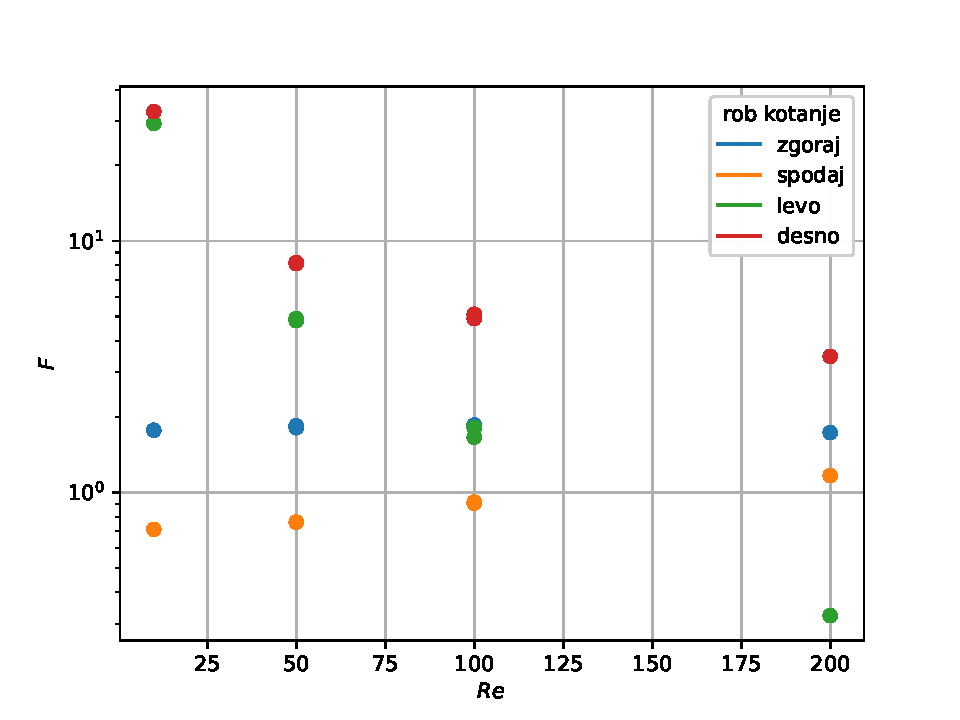
\includegraphics[width=\linewidth]{12.nal_slike/F_Re.pdf}
        \caption{od $Re$ pri fiksnem $N_{iter} = 2000$ in $N_{KV}$ = 2500}
    \end{subfigure}
    \begin{subfigure}{0.49\textwidth}
        \centering
        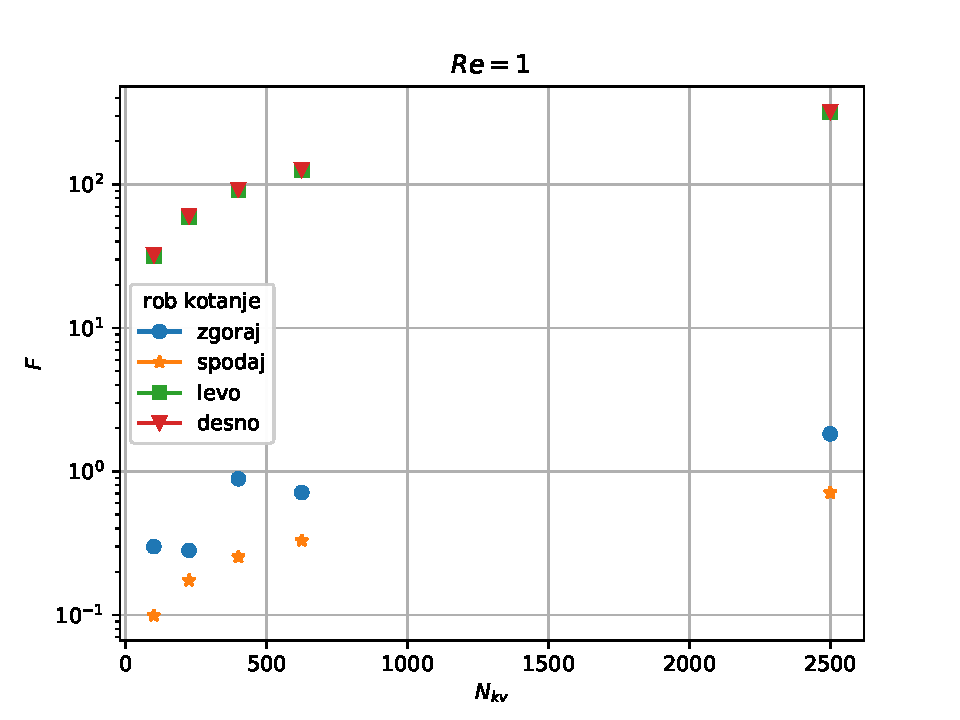
\includegraphics[width=\linewidth]{12.nal_slike/F_Nkv.pdf}
        \caption{od $N_{KV}$ pri fiksnem $Re=1$ in $N_{iter}$ do $10^{-2}$}
    \end{subfigure}
    \begin{subfigure}{0.49\textwidth}
        \centering
        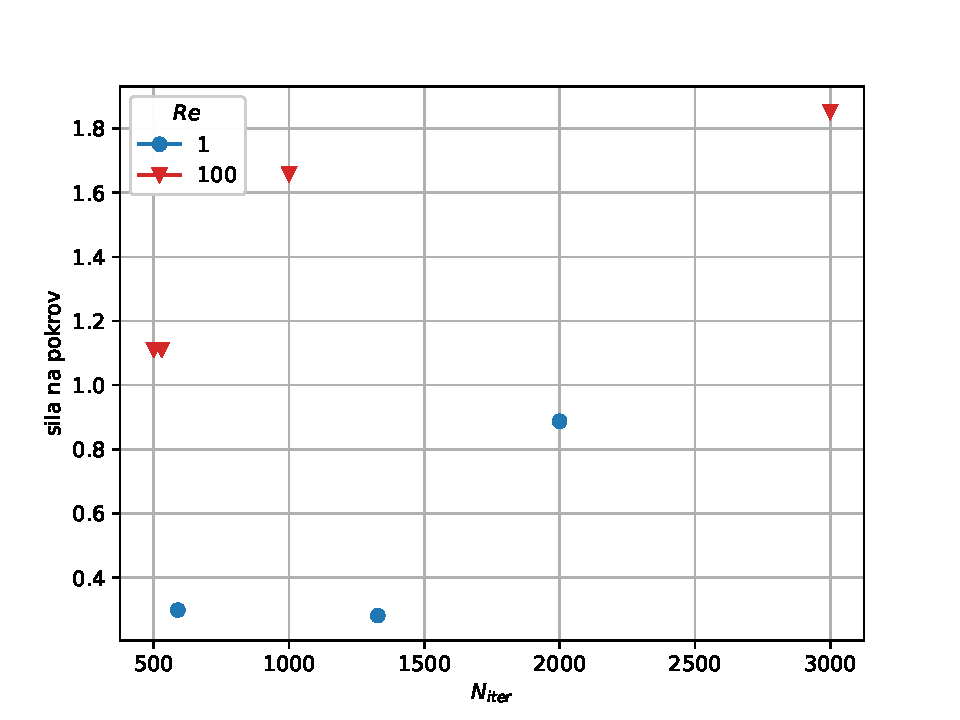
\includegraphics[width=\linewidth]{12.nal_slike/F_Niter.pdf}
        \caption{od $N_{iter}$ pri $N_{KV}=2500$}
    \end{subfigure}
    \caption{Odvinsosti sil na robove od parametrov simulacije}
\end{figure}

\section{Komercialni program}

Enake primere sem izračunal tudi s programom \texttt{Ansys Fluent 2024 R1} in dobil primerljive rezultate. Ker nisem tako vešč dela v tem programu, mi ni uspelo prikazati tokovnic, zato je tu vektorsko polje hitrosti. Uporabil sem algoritem SIMPLE in privetrno diskretizacijsko shemo momentne enačbe prvega reda ter enak začetni približek, vendar pa vseh parametrov ni mogoče uskladiti s simulacijo. Prav tako je izračun tukaj mnogo hitrejši, predvsem pa bolje konvergira.

\begin{figure}[H]
    \centering
    \begin{subfigure}{0.49\textwidth}
        \centering
        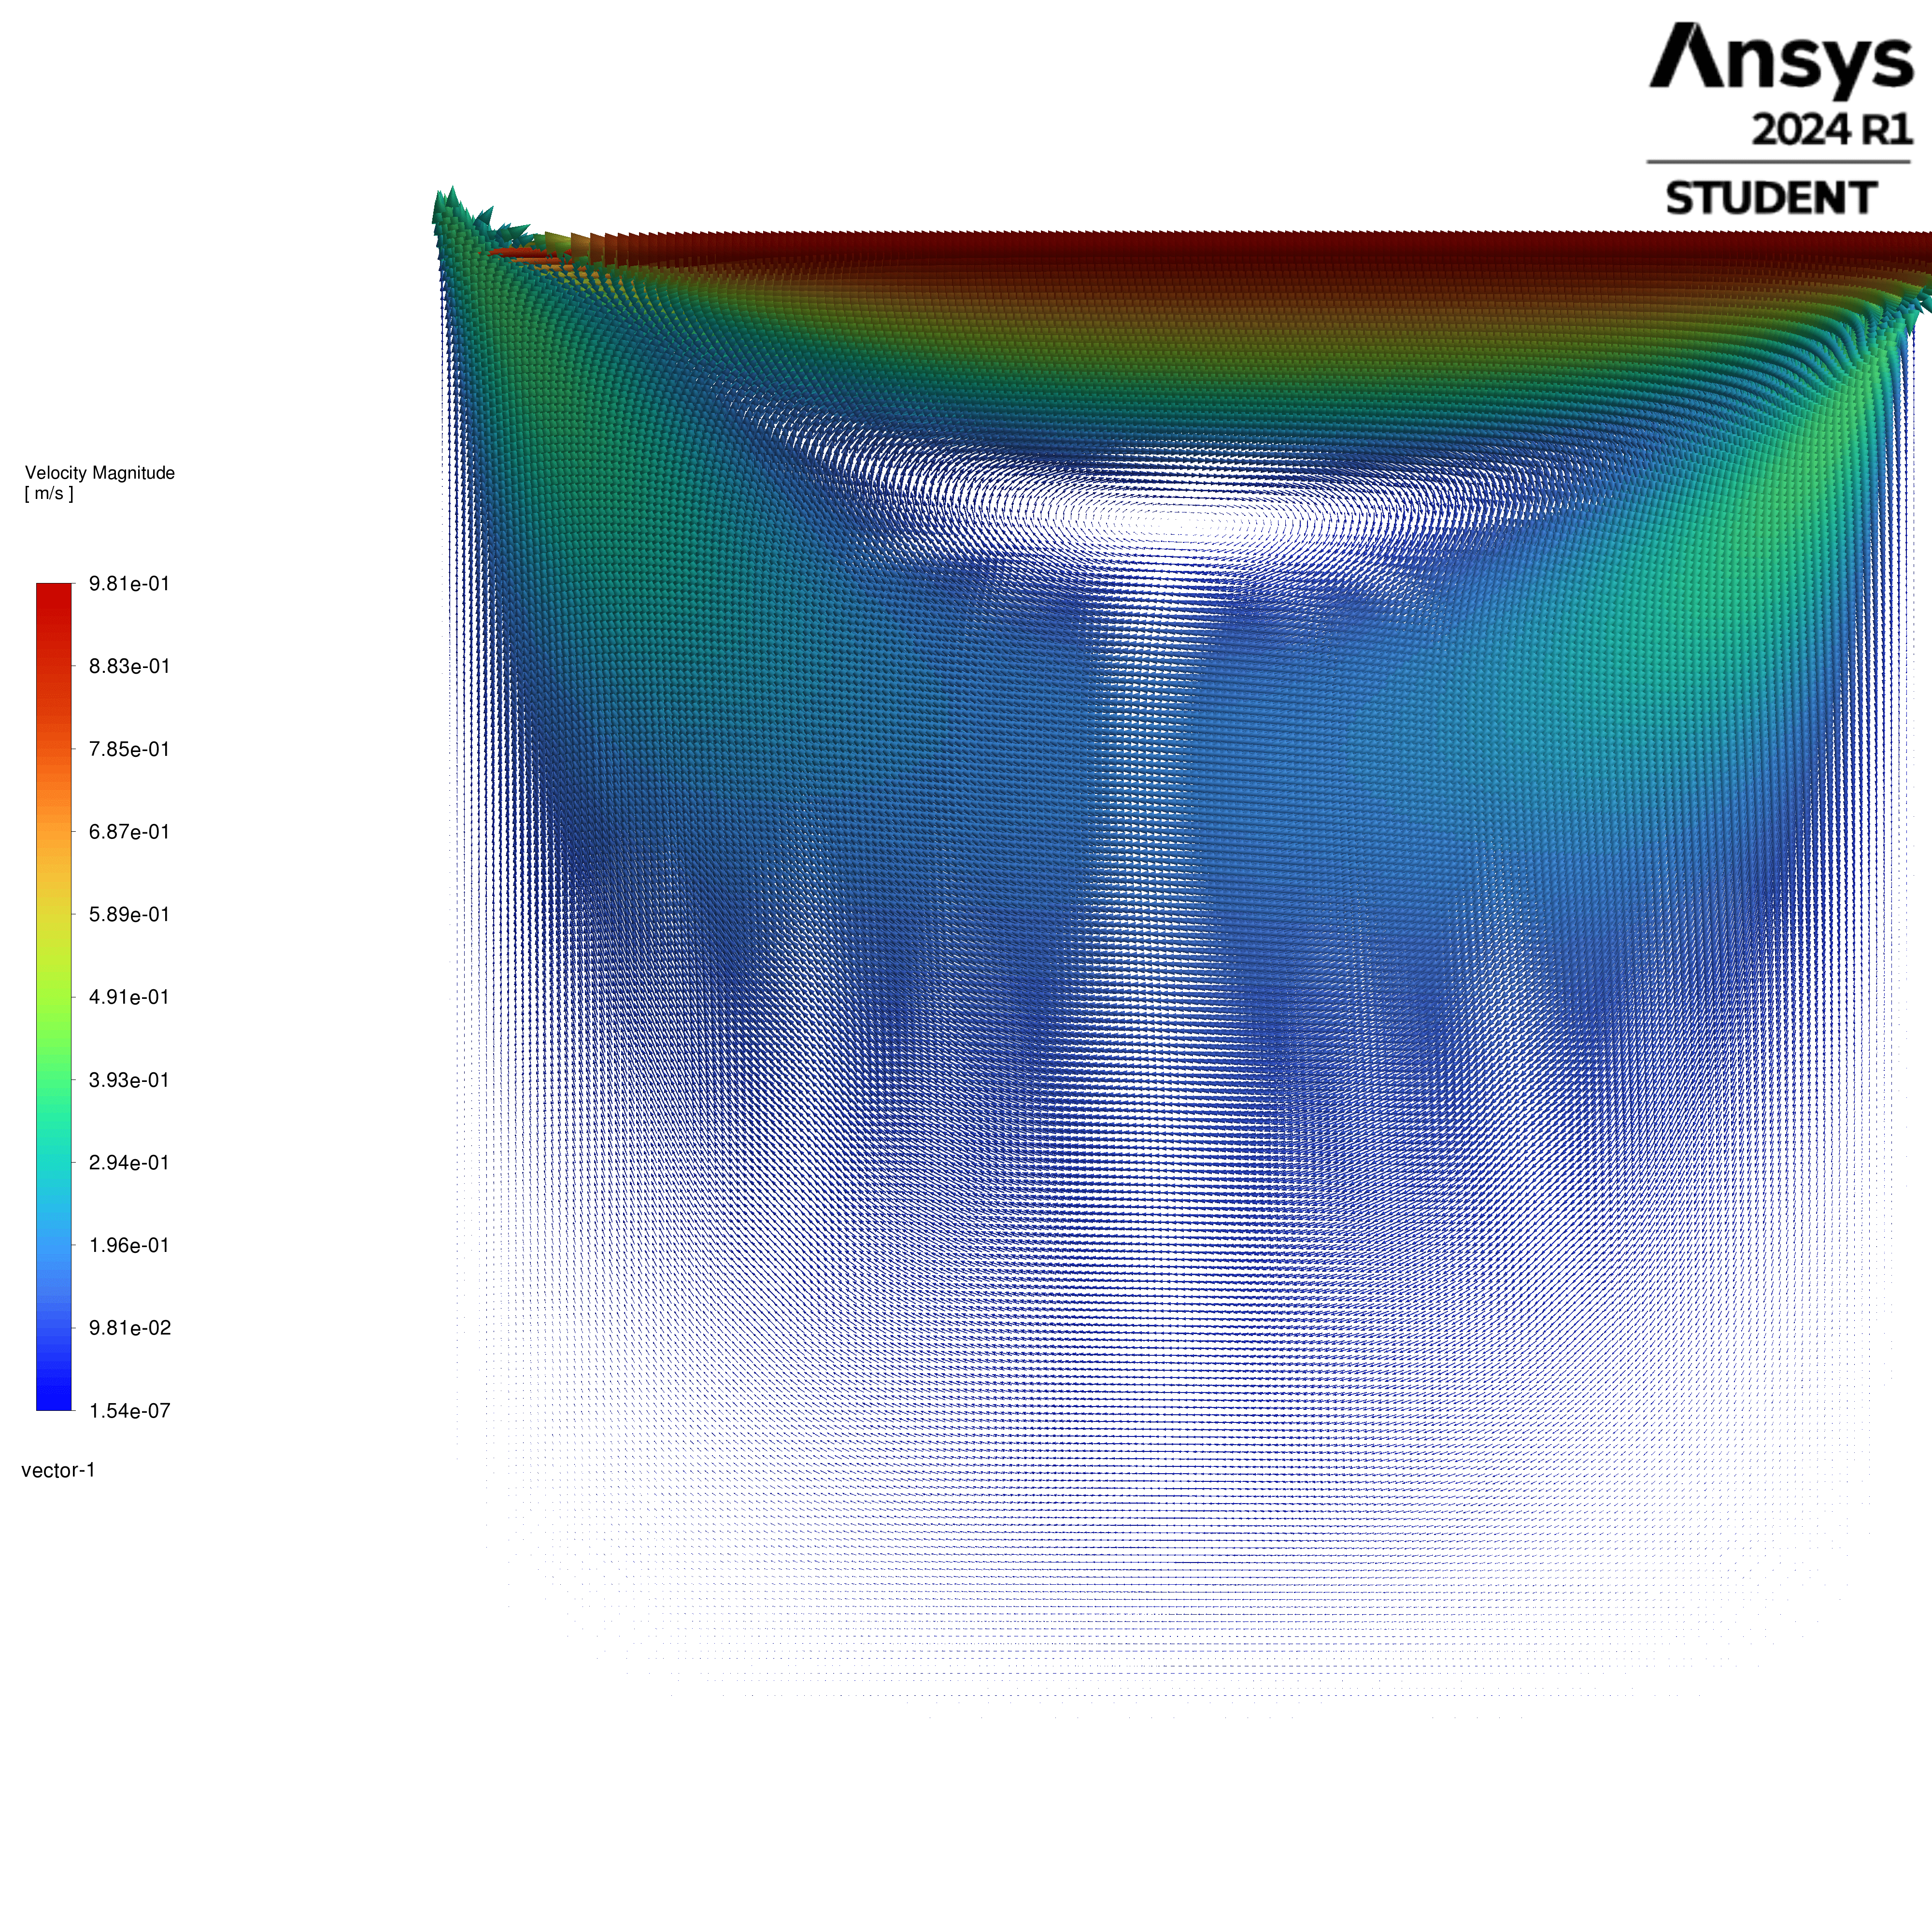
\includegraphics[width=\linewidth]{12.nal_slike/ansys/Re1_v-min.png}
        \caption{hitrostno polje}
    \end{subfigure}
    \begin{subfigure}{0.49\textwidth}
        \centering
        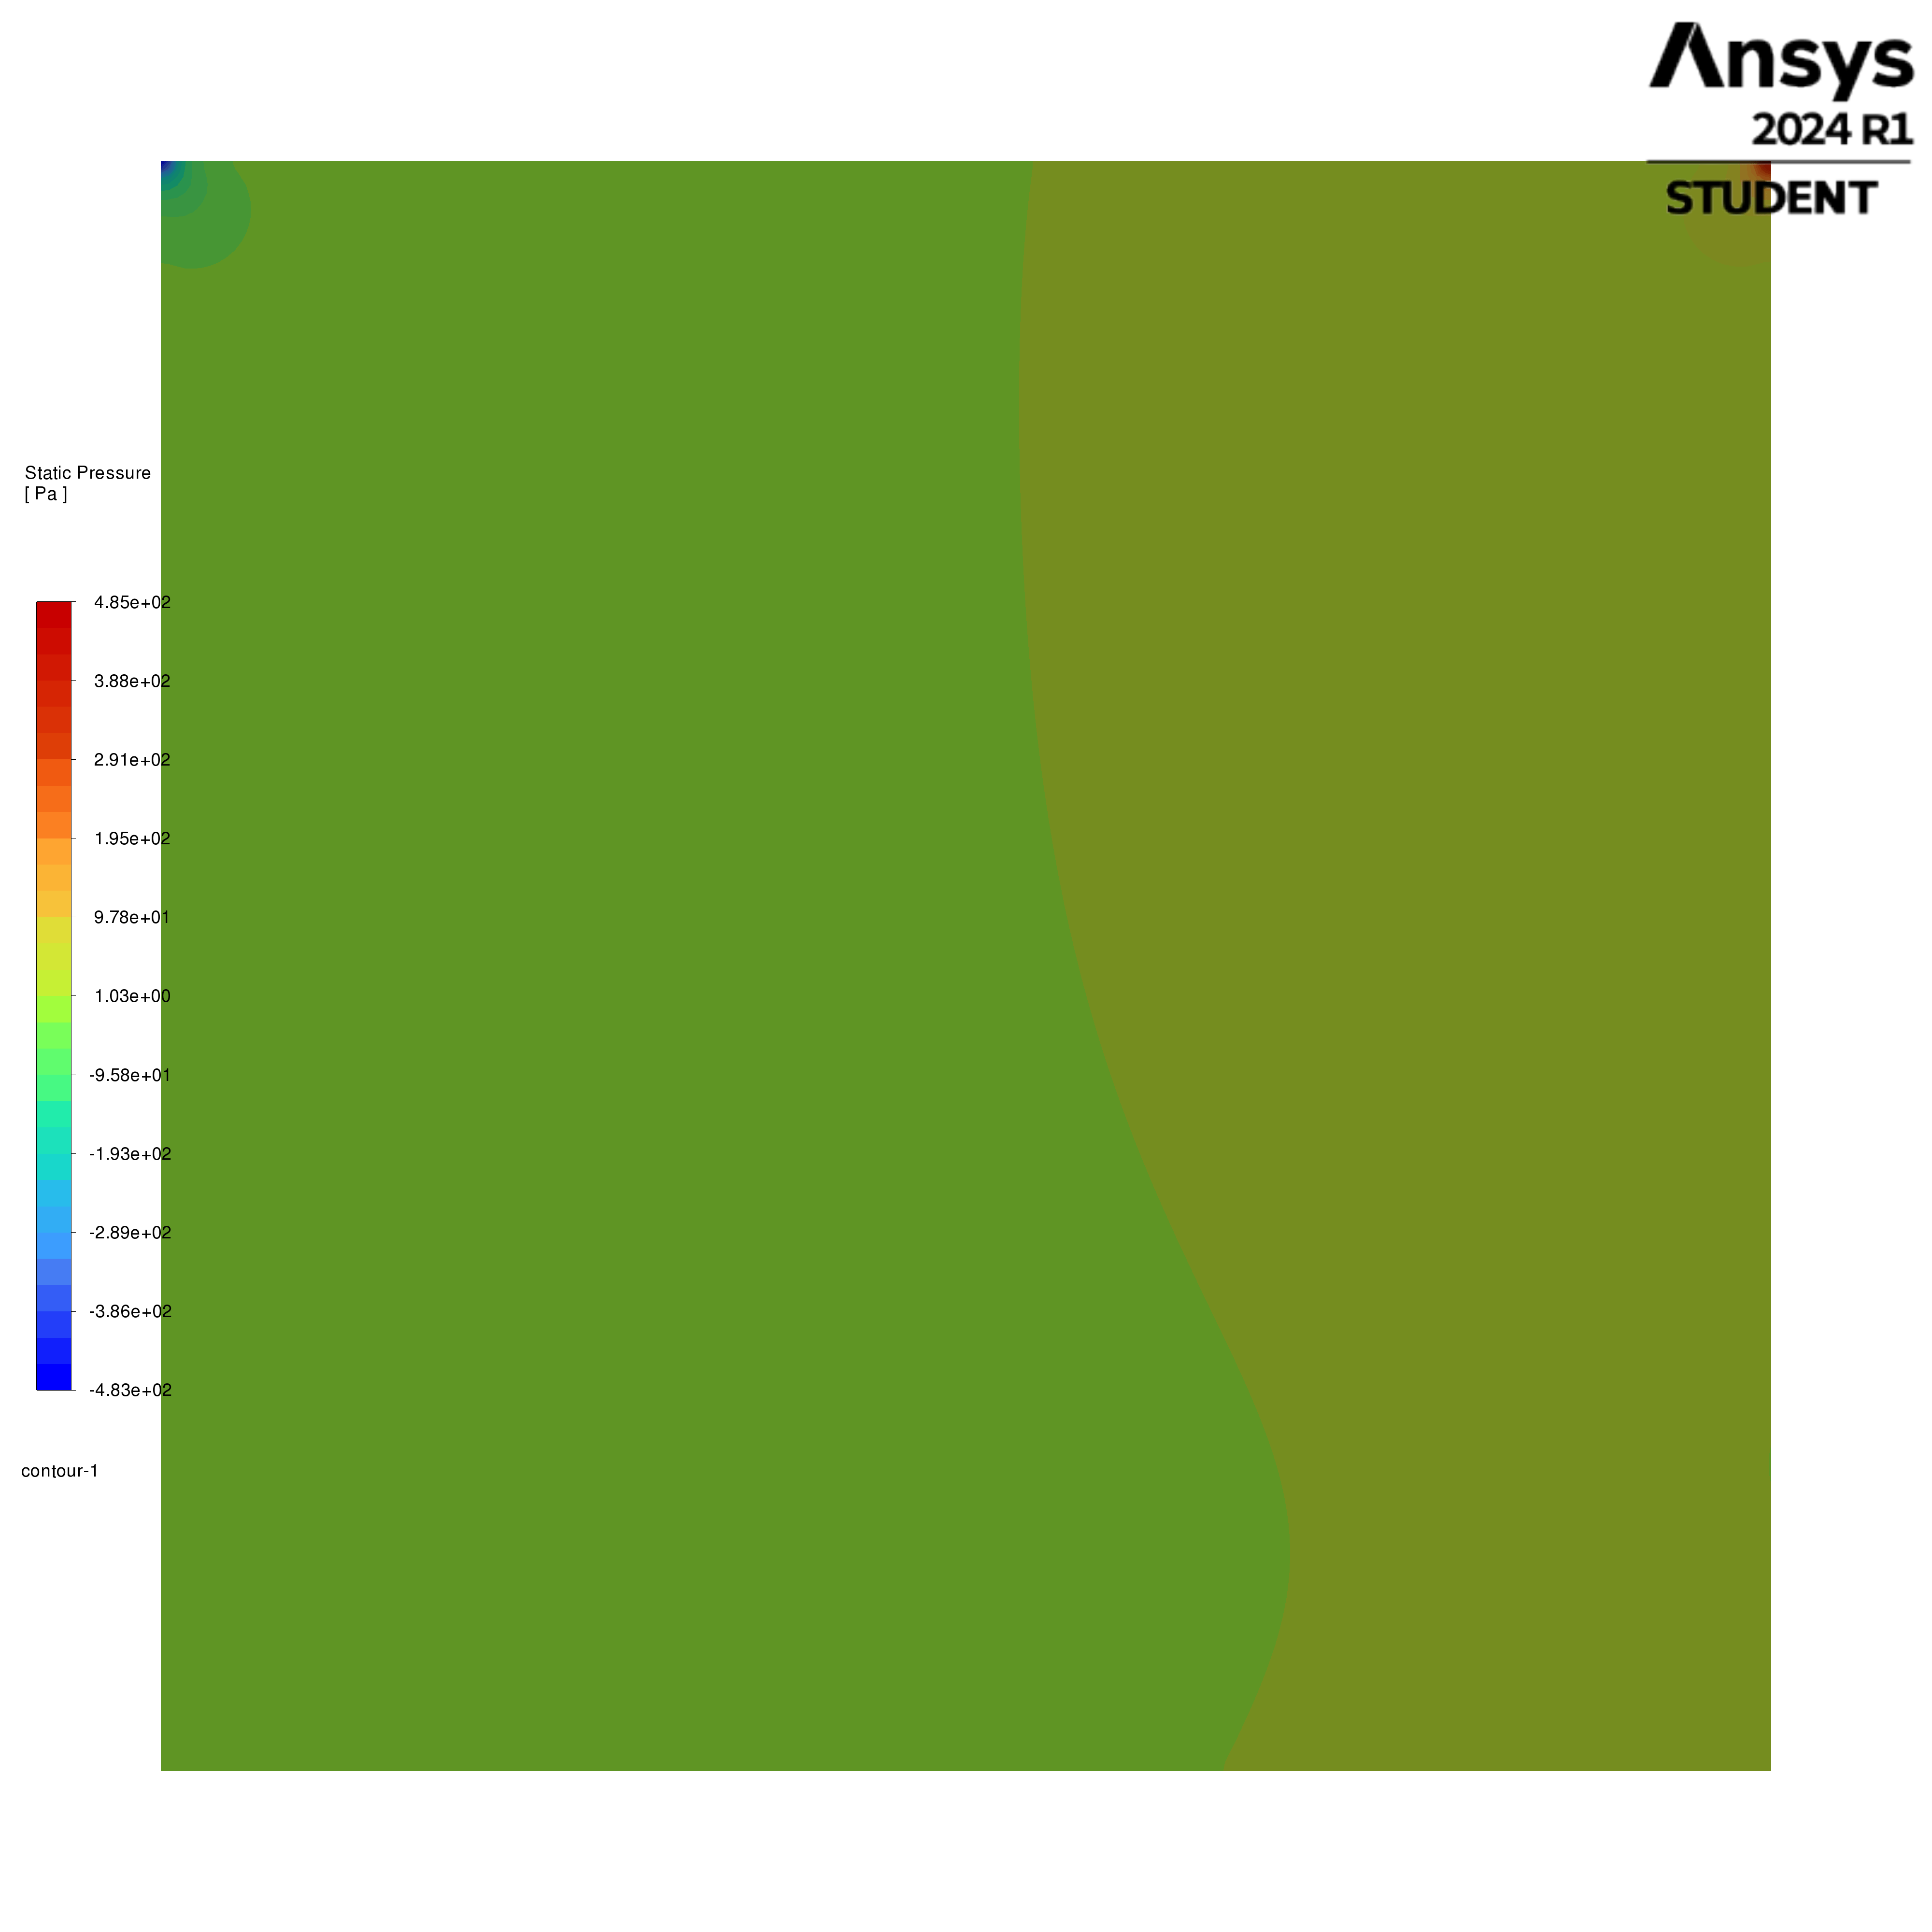
\includegraphics[width=\linewidth]{12.nal_slike/ansys/Re1_p-min.png}
        \caption{tlačno polje}
    \end{subfigure}
    \begin{subfigure}{\textwidth}
        \centering
        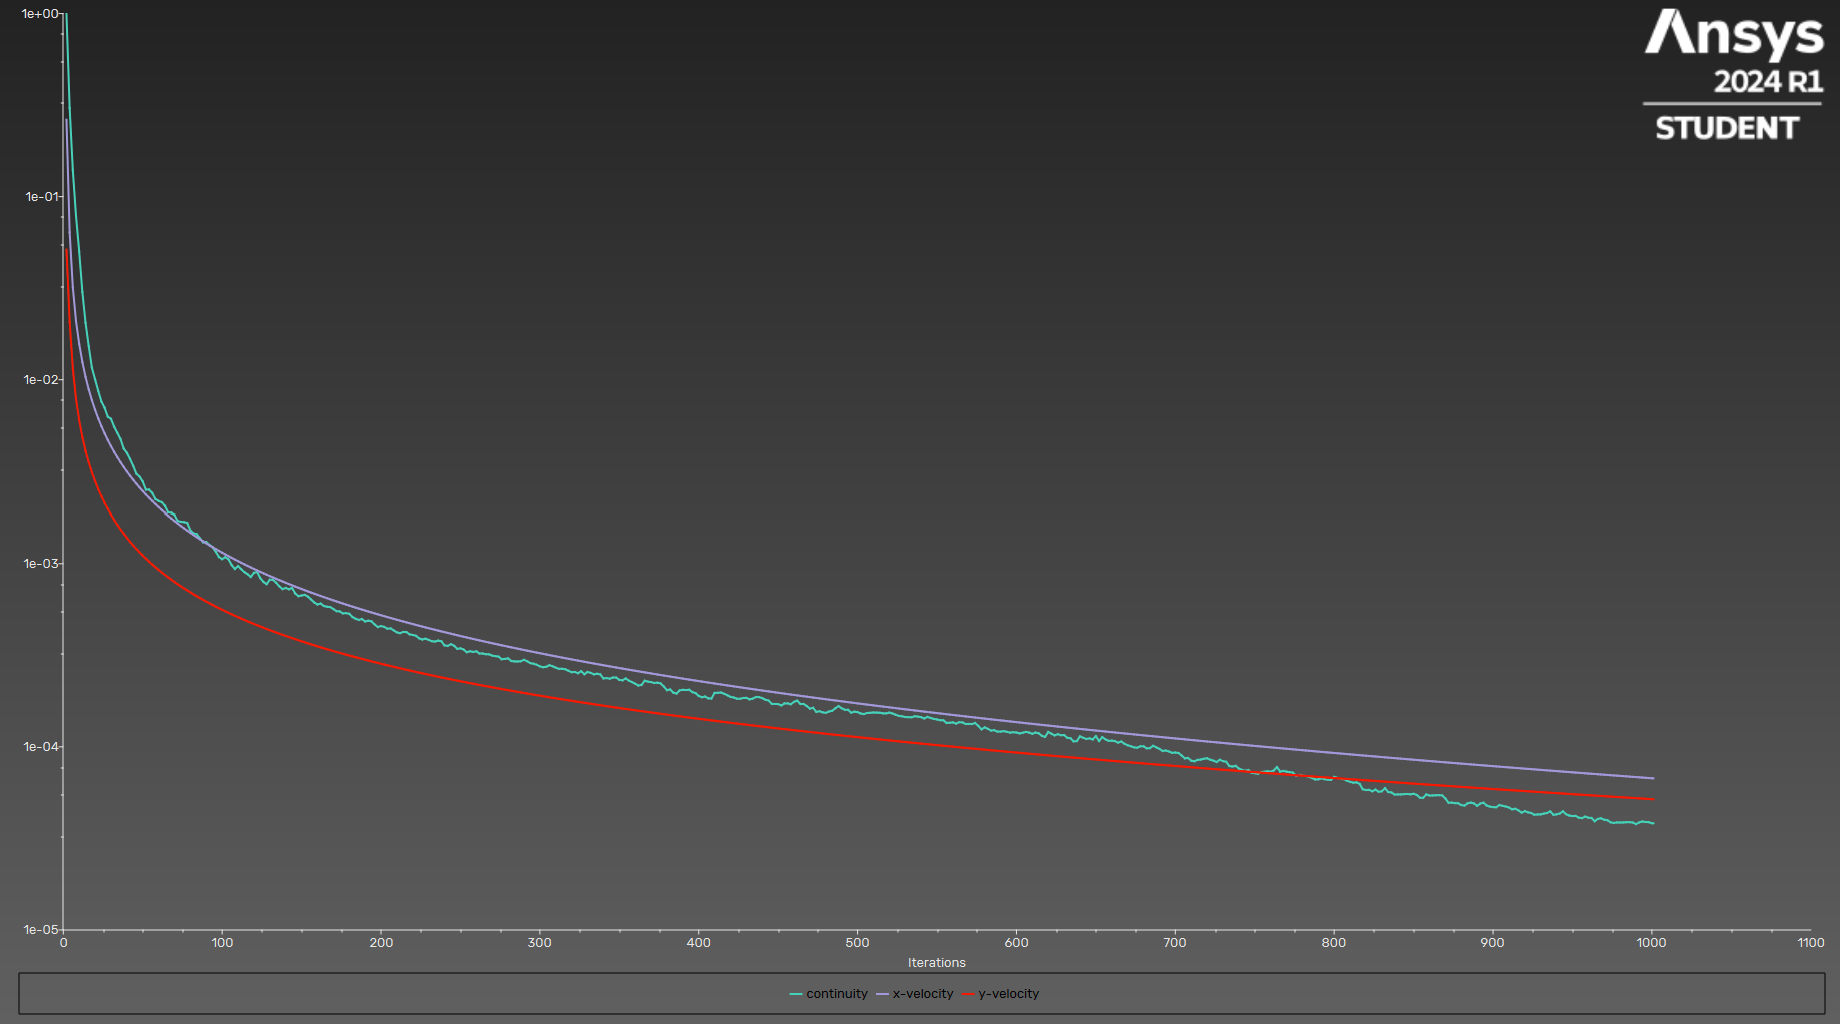
\includegraphics[width=\linewidth]{12.nal_slike/ansys/Re1-min.png}
        \caption{konvergenca residualov}
    \end{subfigure}
    \caption{$Re=1$}
\end{figure}

\begin{figure}[H]
    \centering
    \begin{subfigure}{0.49\textwidth}
        \centering
        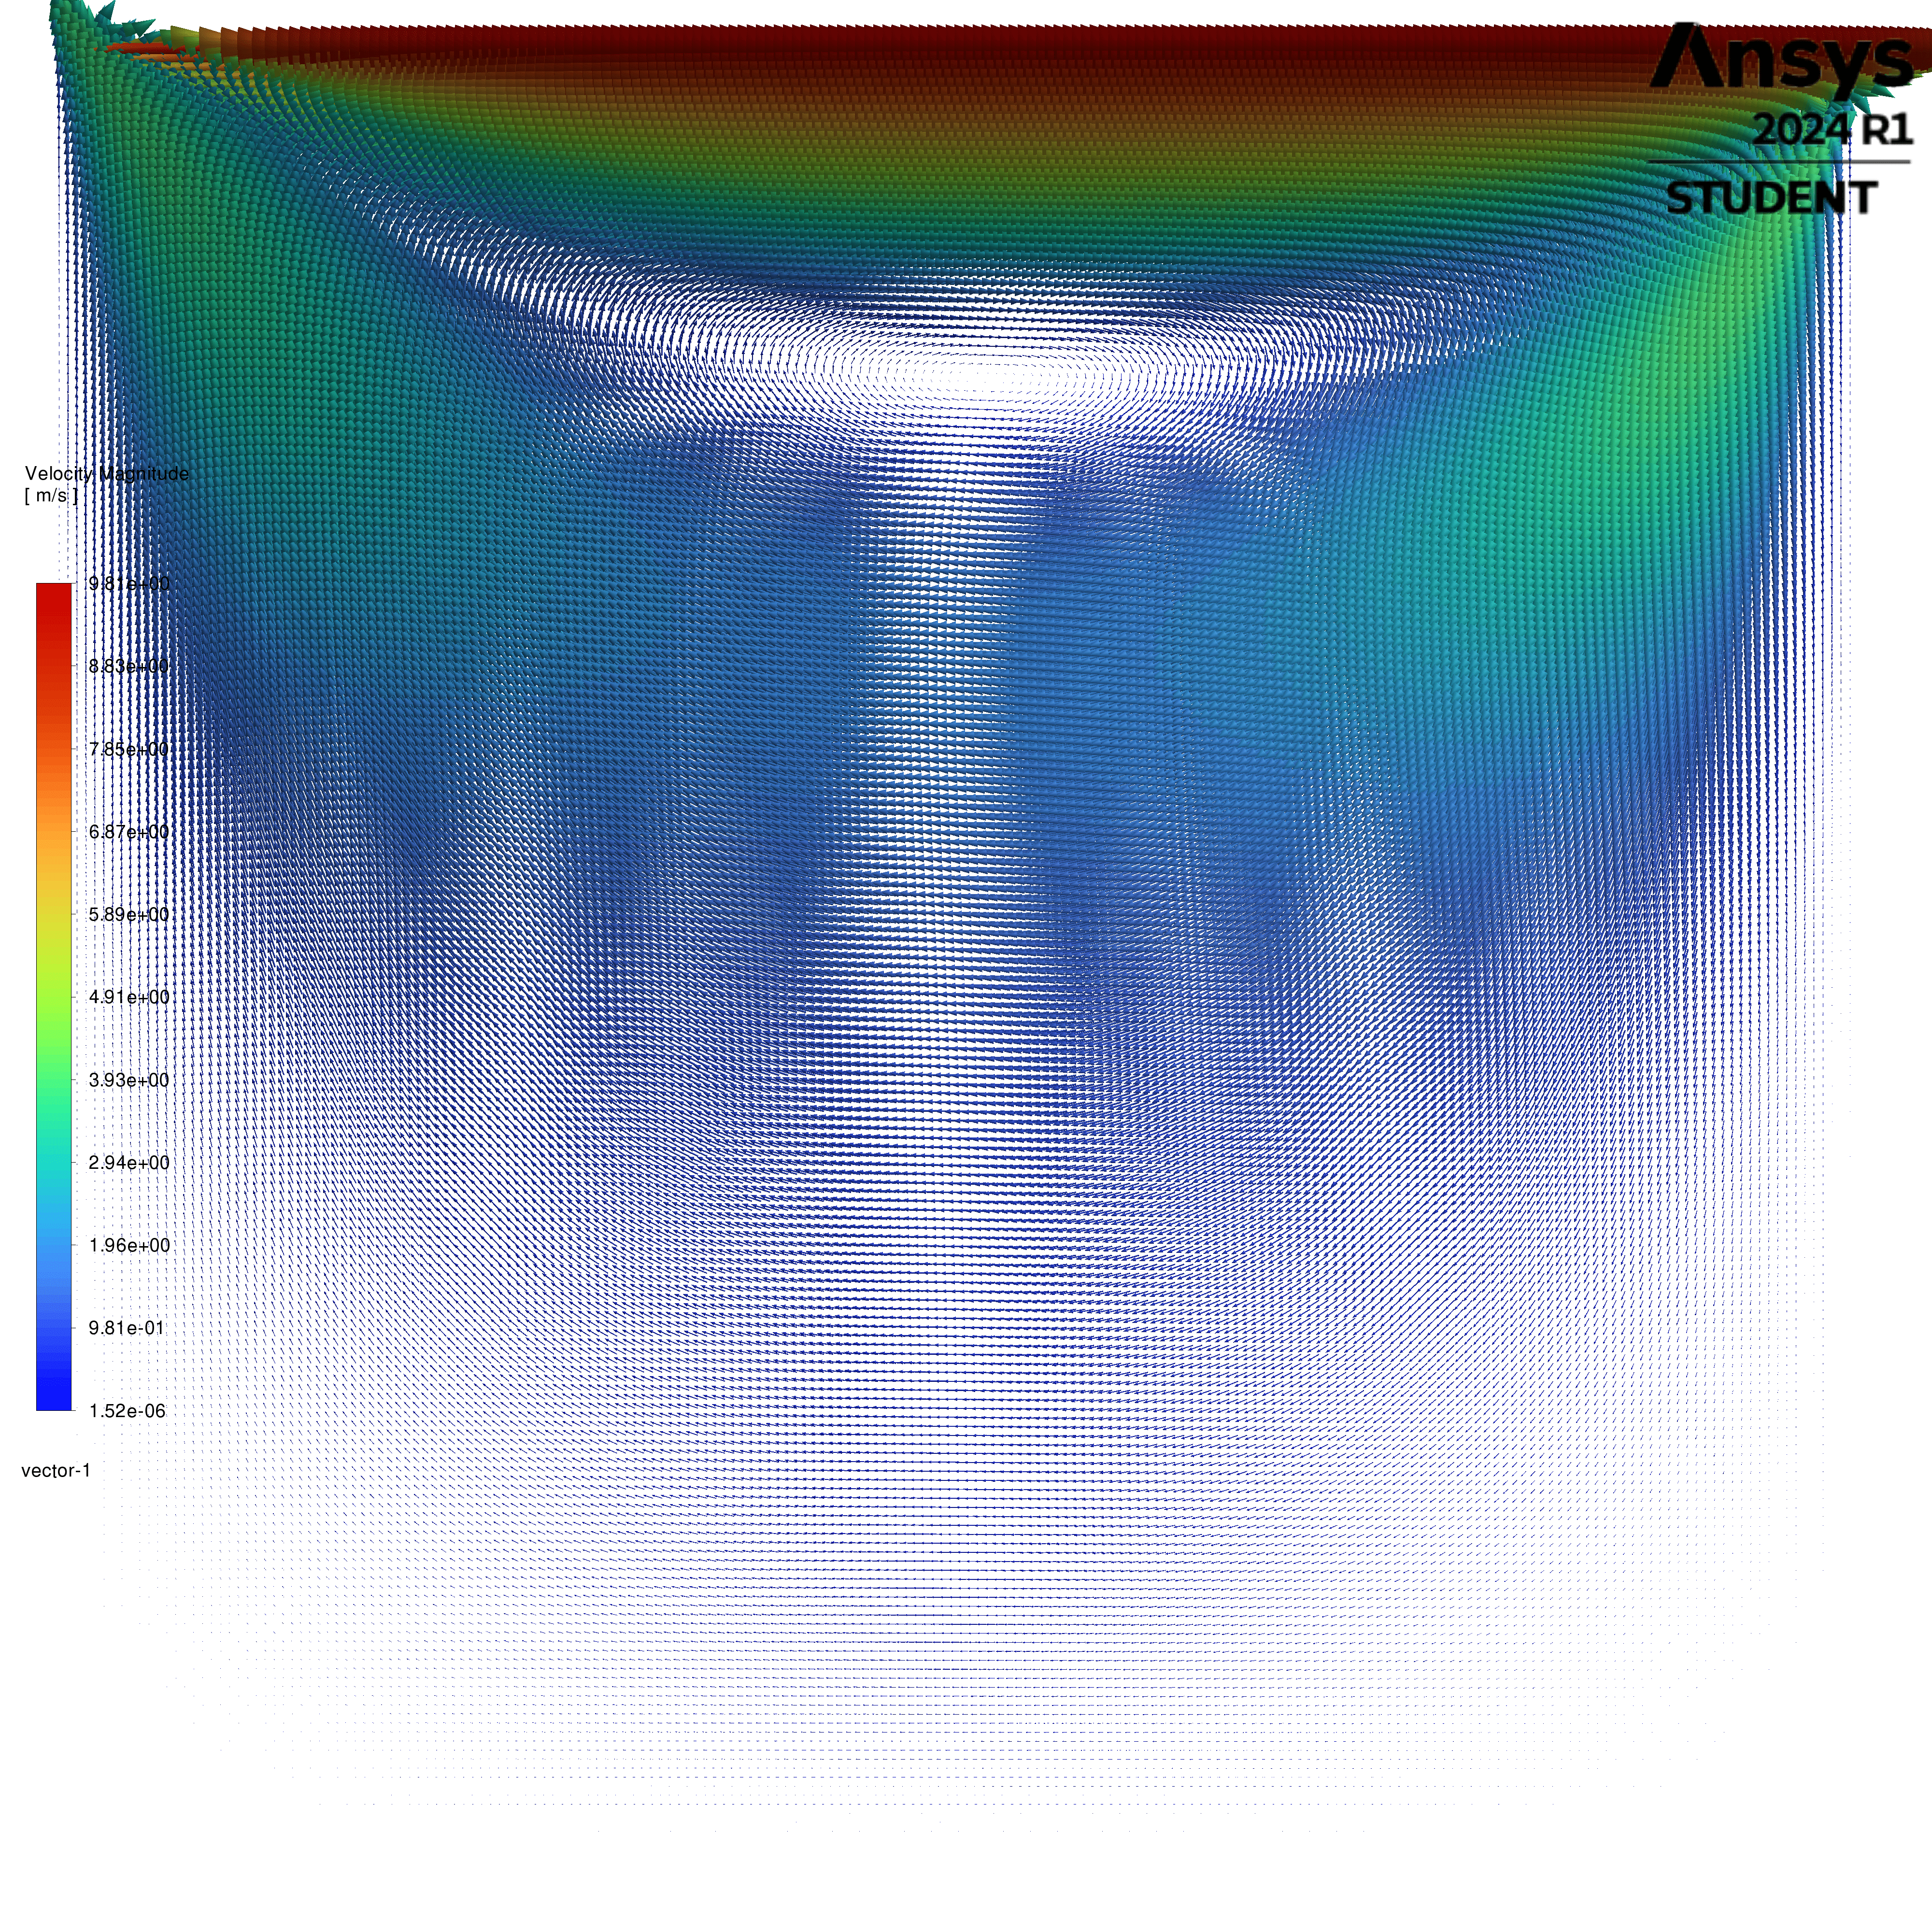
\includegraphics[width=\linewidth]{12.nal_slike/ansys/Re10_v-min.png}
        \caption{hitrostno polje}
    \end{subfigure}
    \begin{subfigure}{0.49\textwidth}
        \centering
        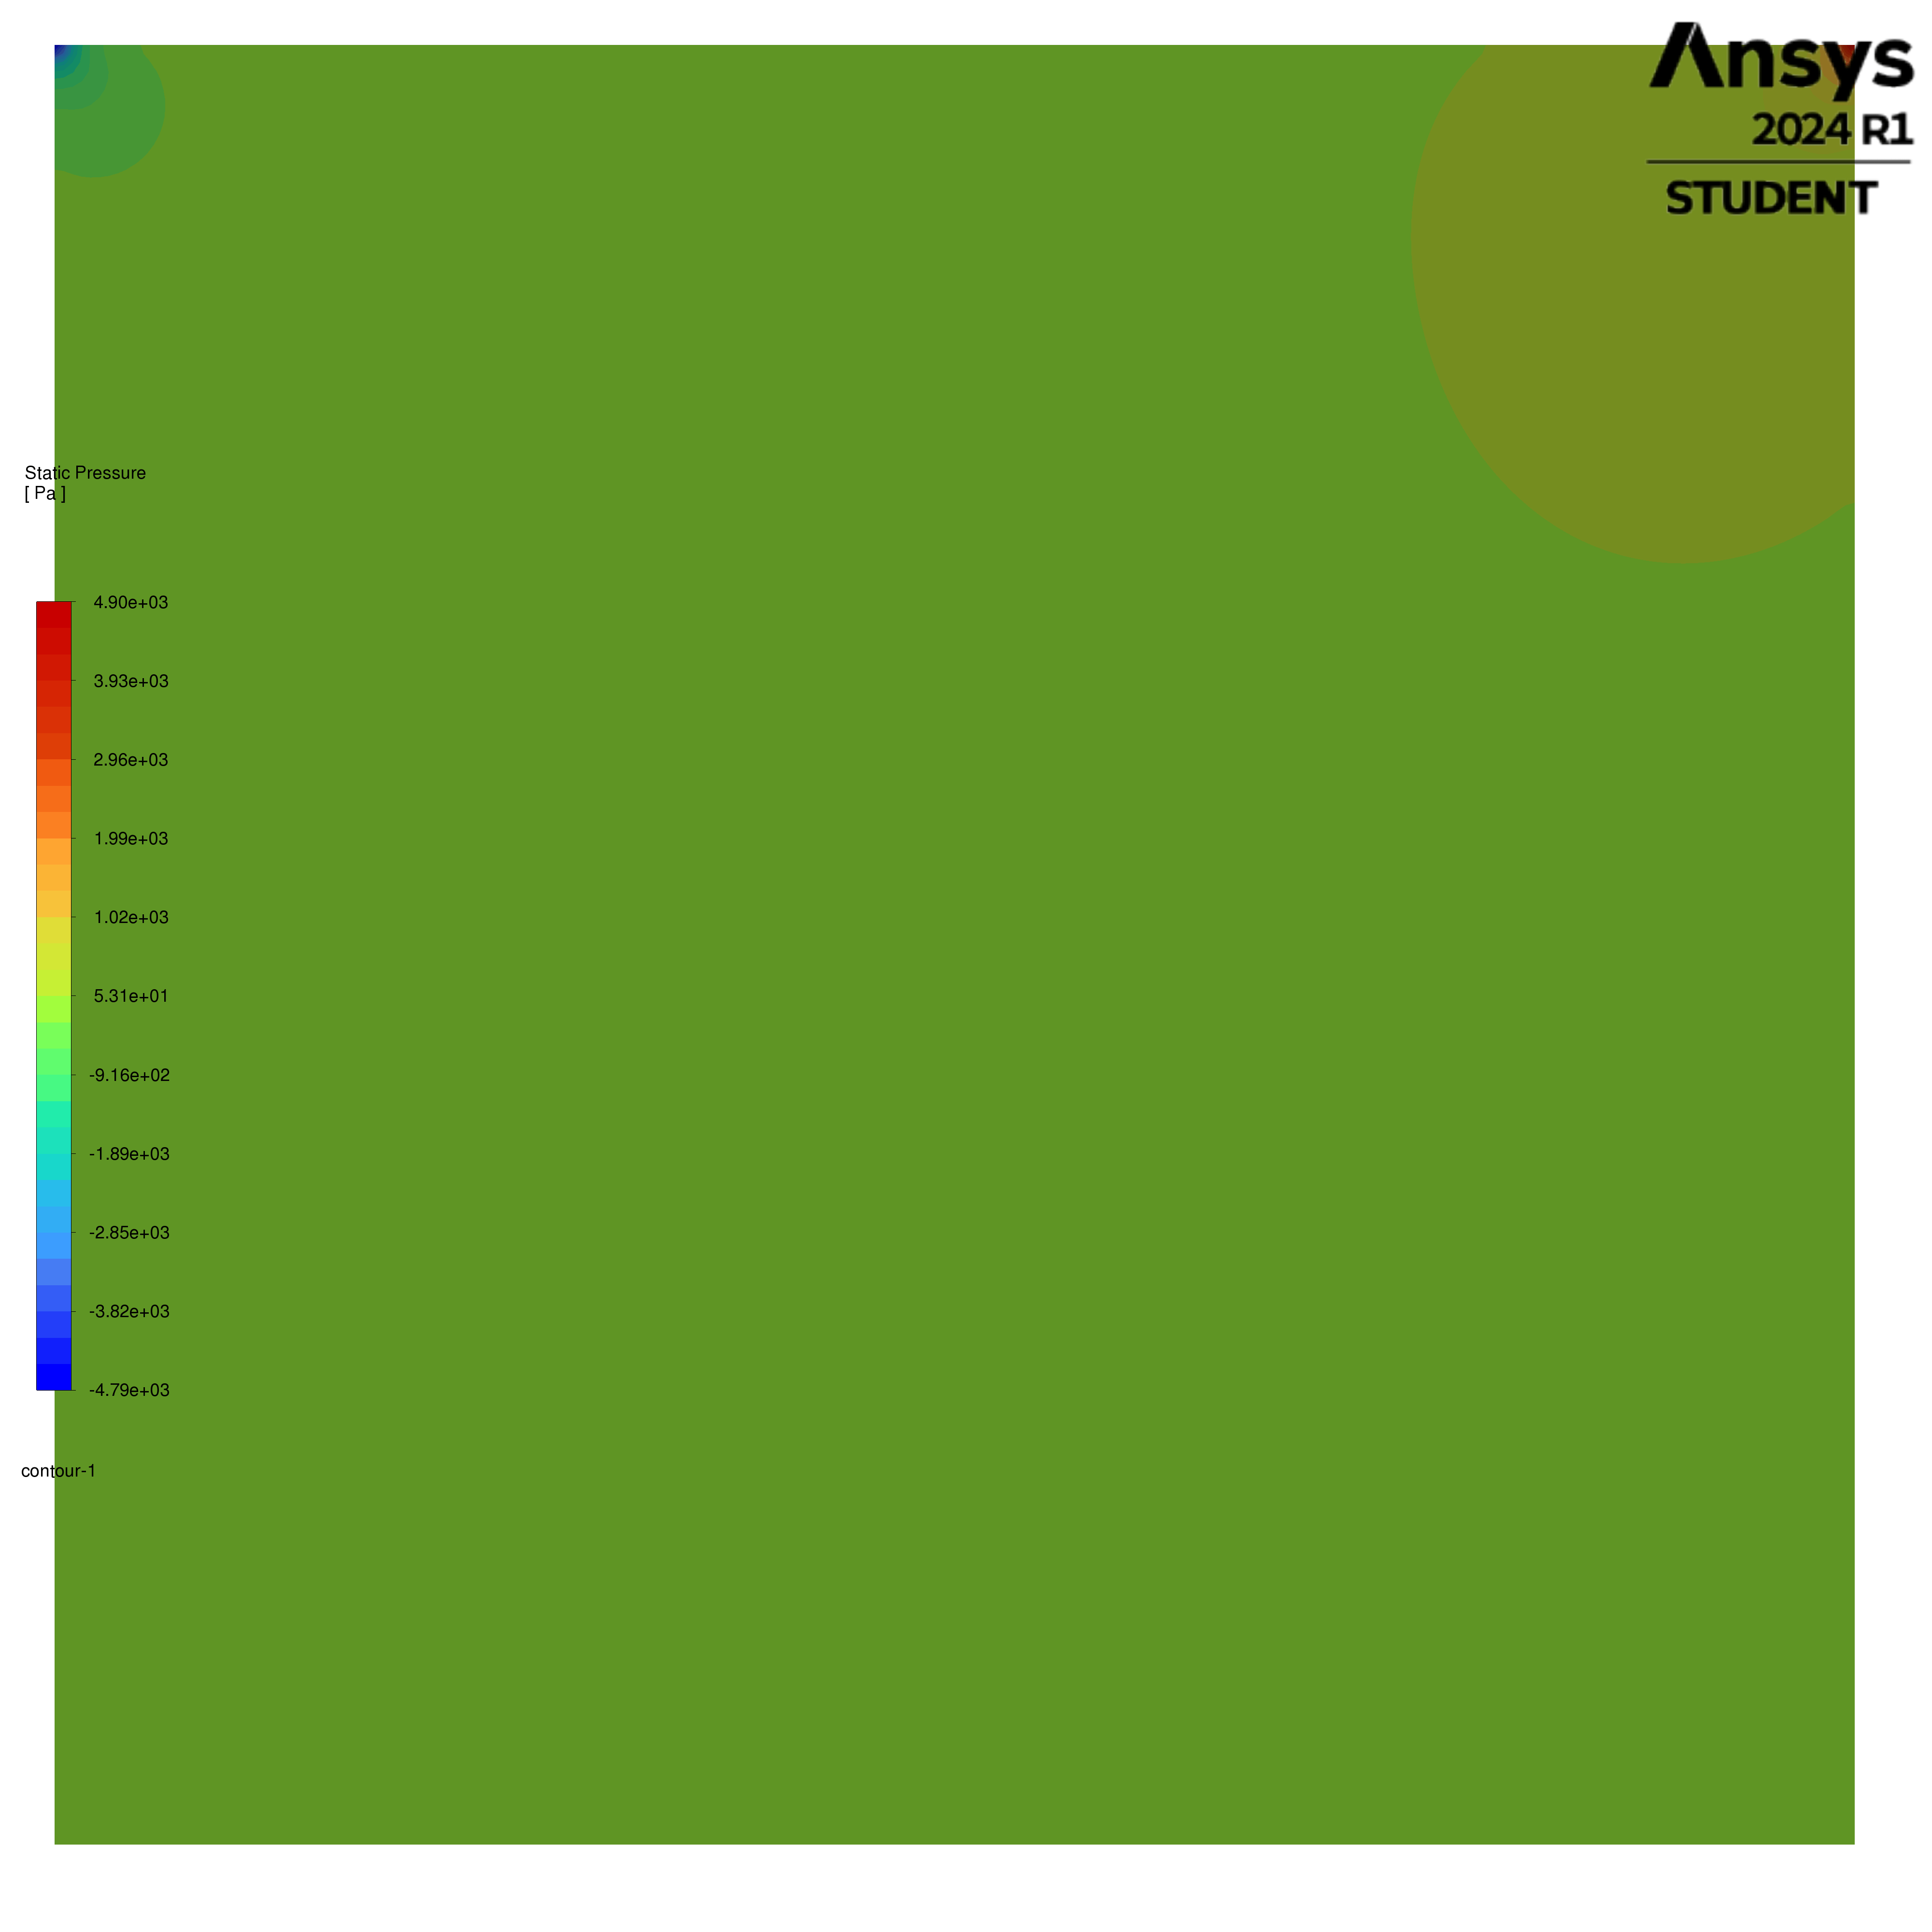
\includegraphics[width=\linewidth]{12.nal_slike/ansys/Re10_p-min.png}
        \caption{tlačno polje}
    \end{subfigure}
    \begin{subfigure}{\textwidth}
        \centering
        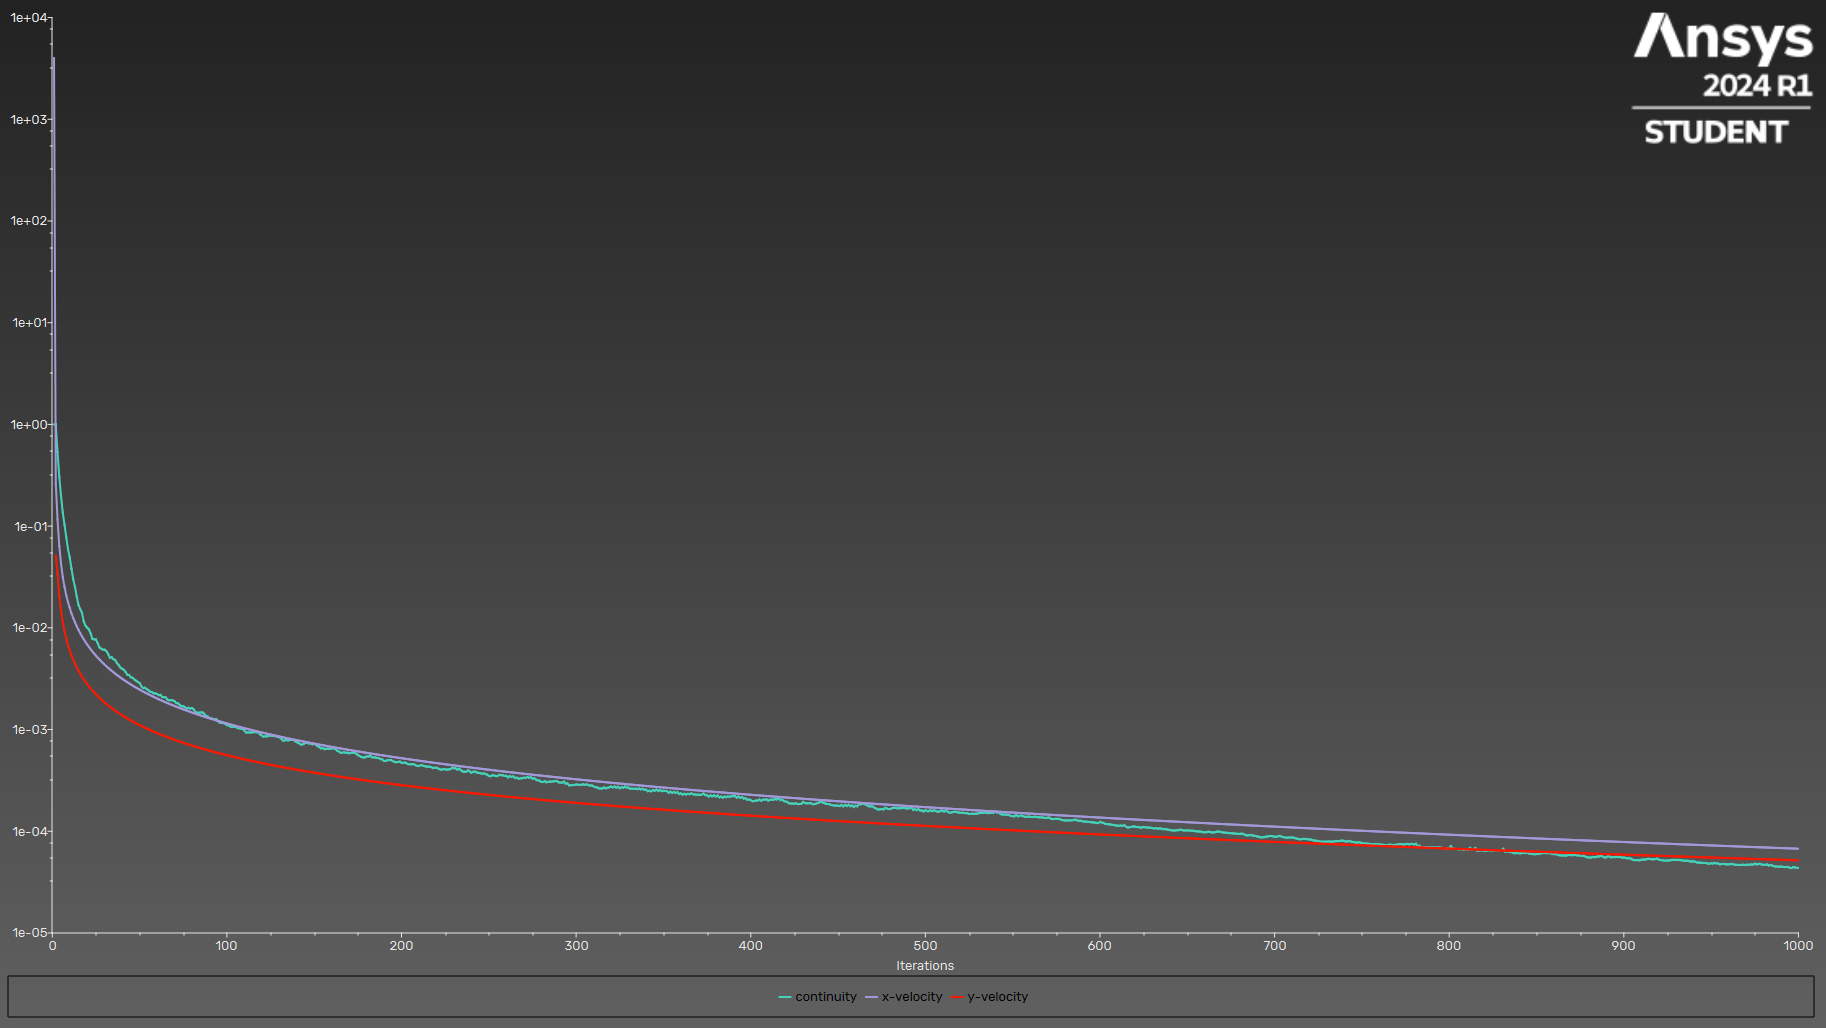
\includegraphics[width=\linewidth]{12.nal_slike/ansys/Re10-min.png}
        \caption{konvergenca residualov}
    \end{subfigure}
    \caption{$Re=10$}
\end{figure}

\begin{figure}[H]
    \centering
    \begin{subfigure}{0.49\textwidth}
        \centering
        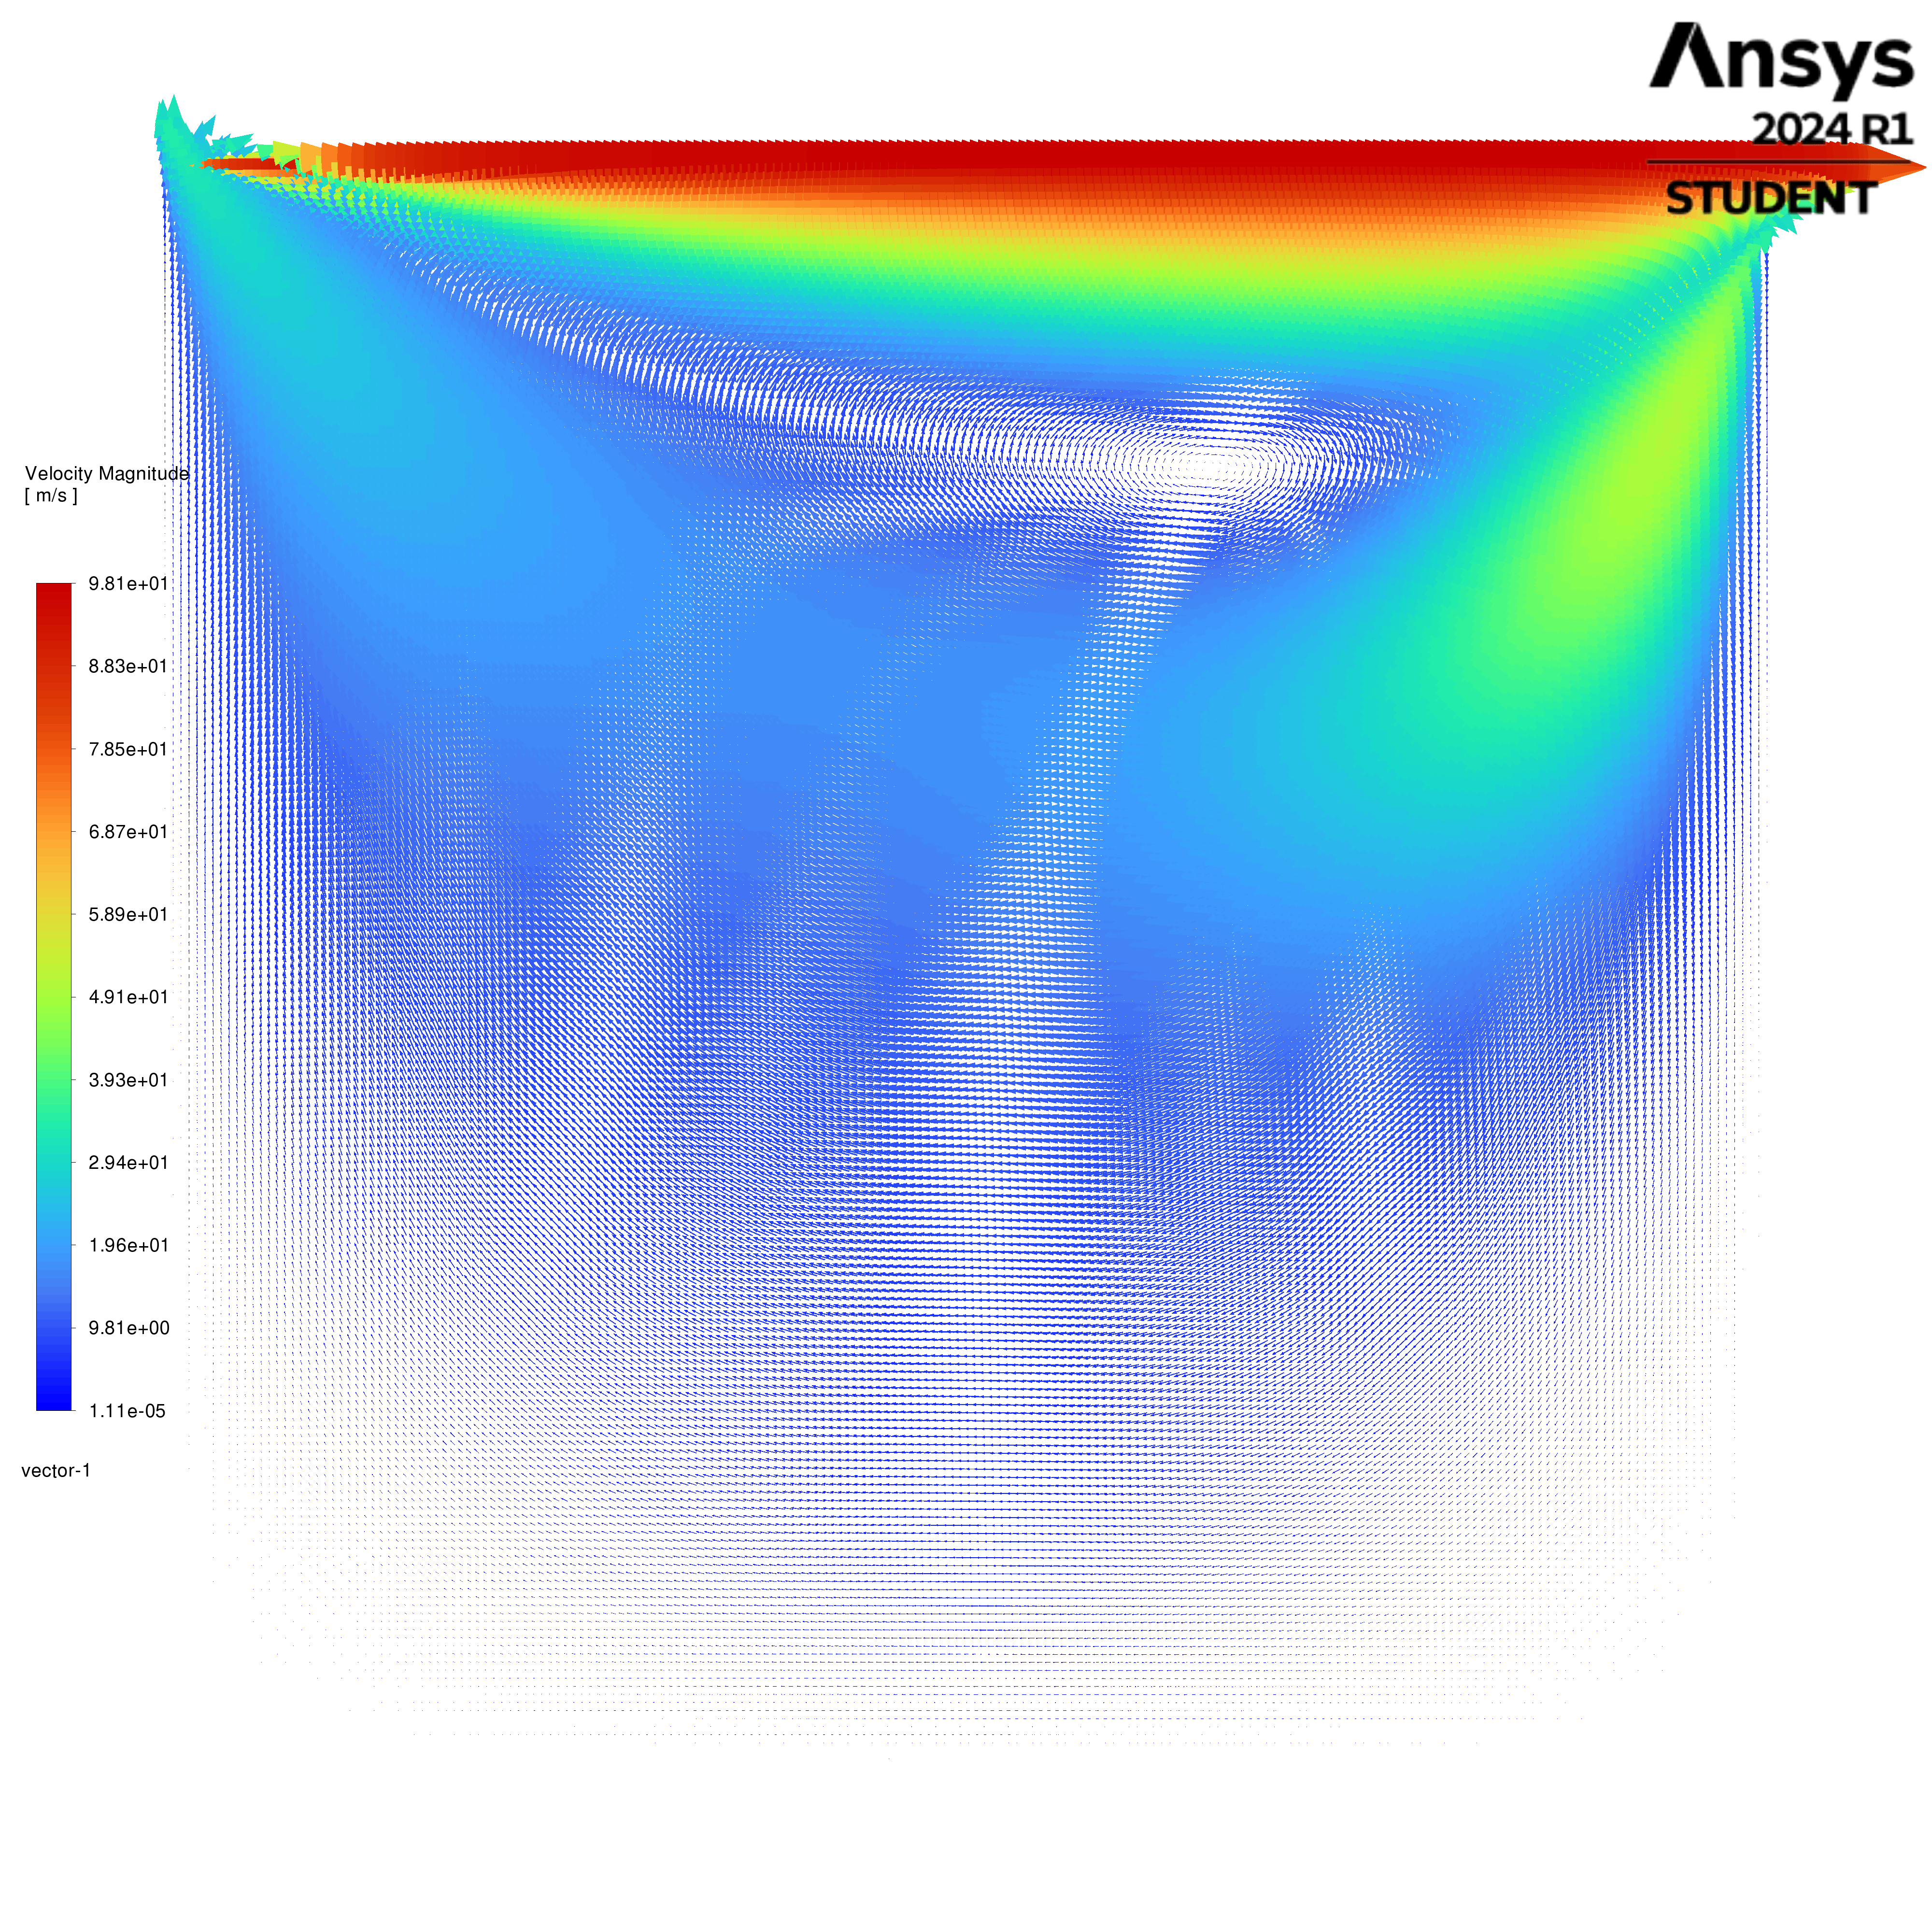
\includegraphics[width=\linewidth]{12.nal_slike/ansys/Re100_v-min.png}
        \caption{hitrostno polje}
    \end{subfigure}
    \begin{subfigure}{0.49\textwidth}
        \centering
        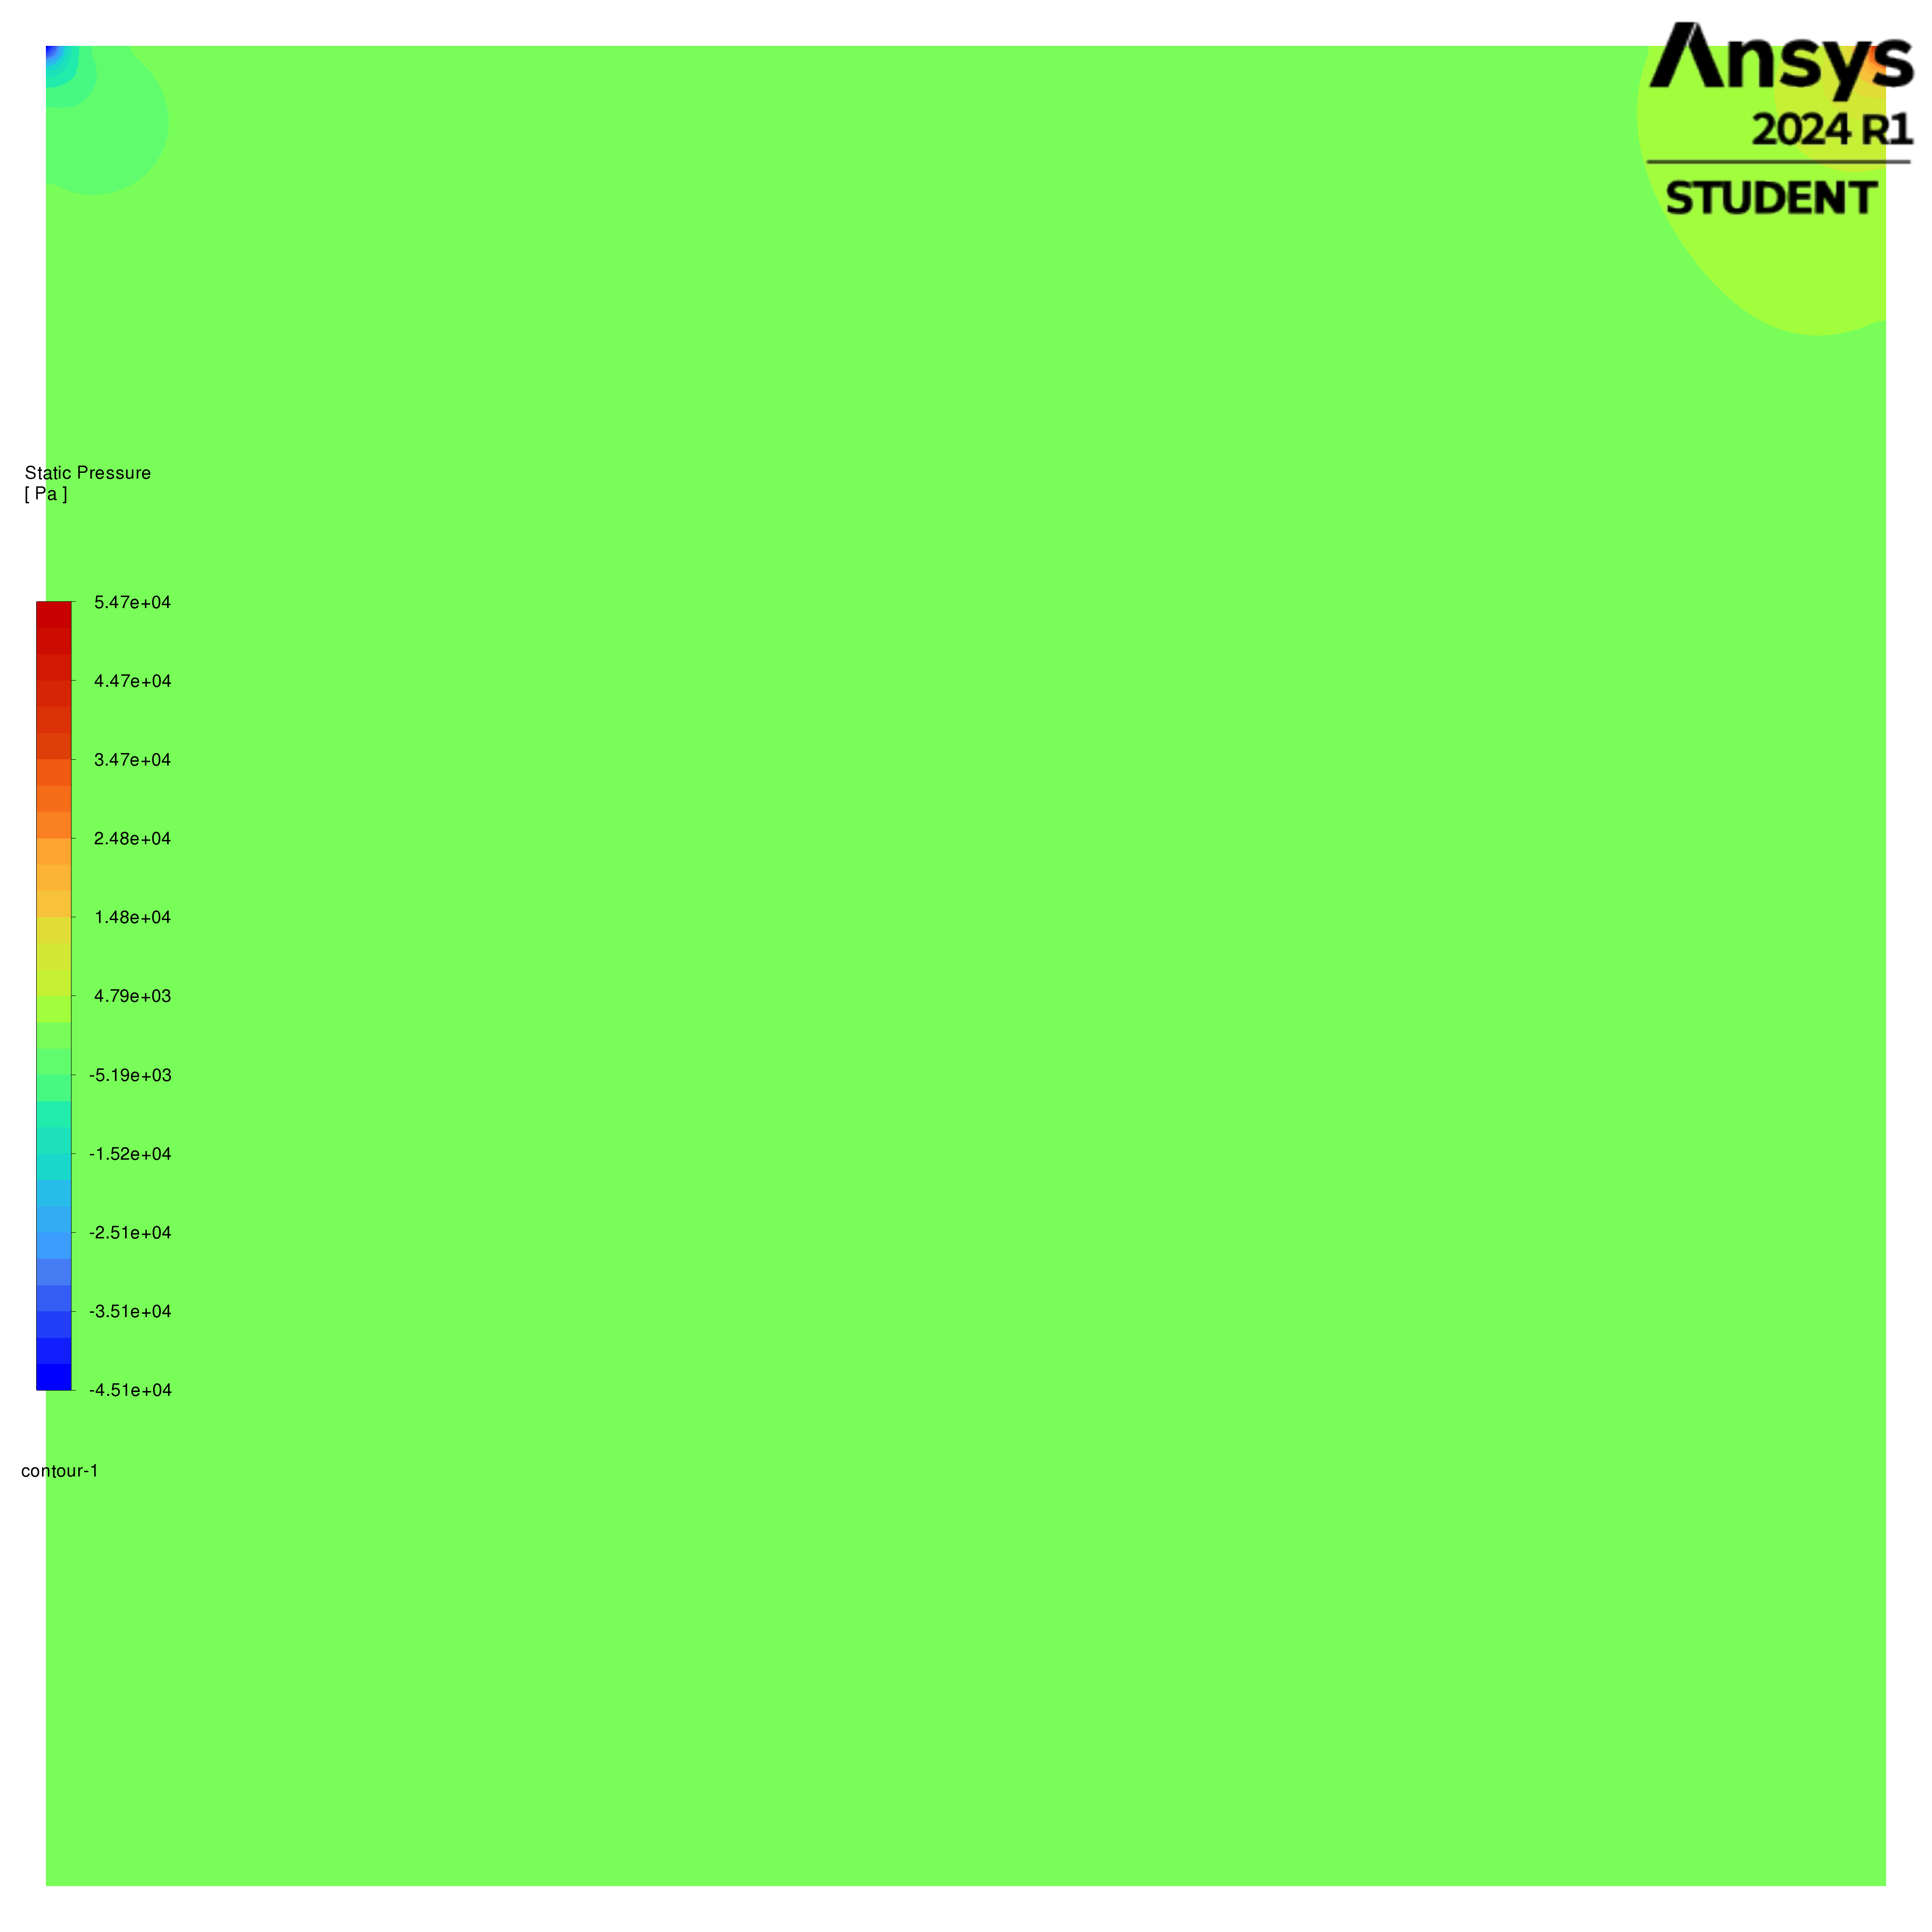
\includegraphics[width=\linewidth]{12.nal_slike/ansys/Re100_p-min.png}
        \caption{tlačno polje}
    \end{subfigure}
    \begin{subfigure}{\textwidth}
        \centering
        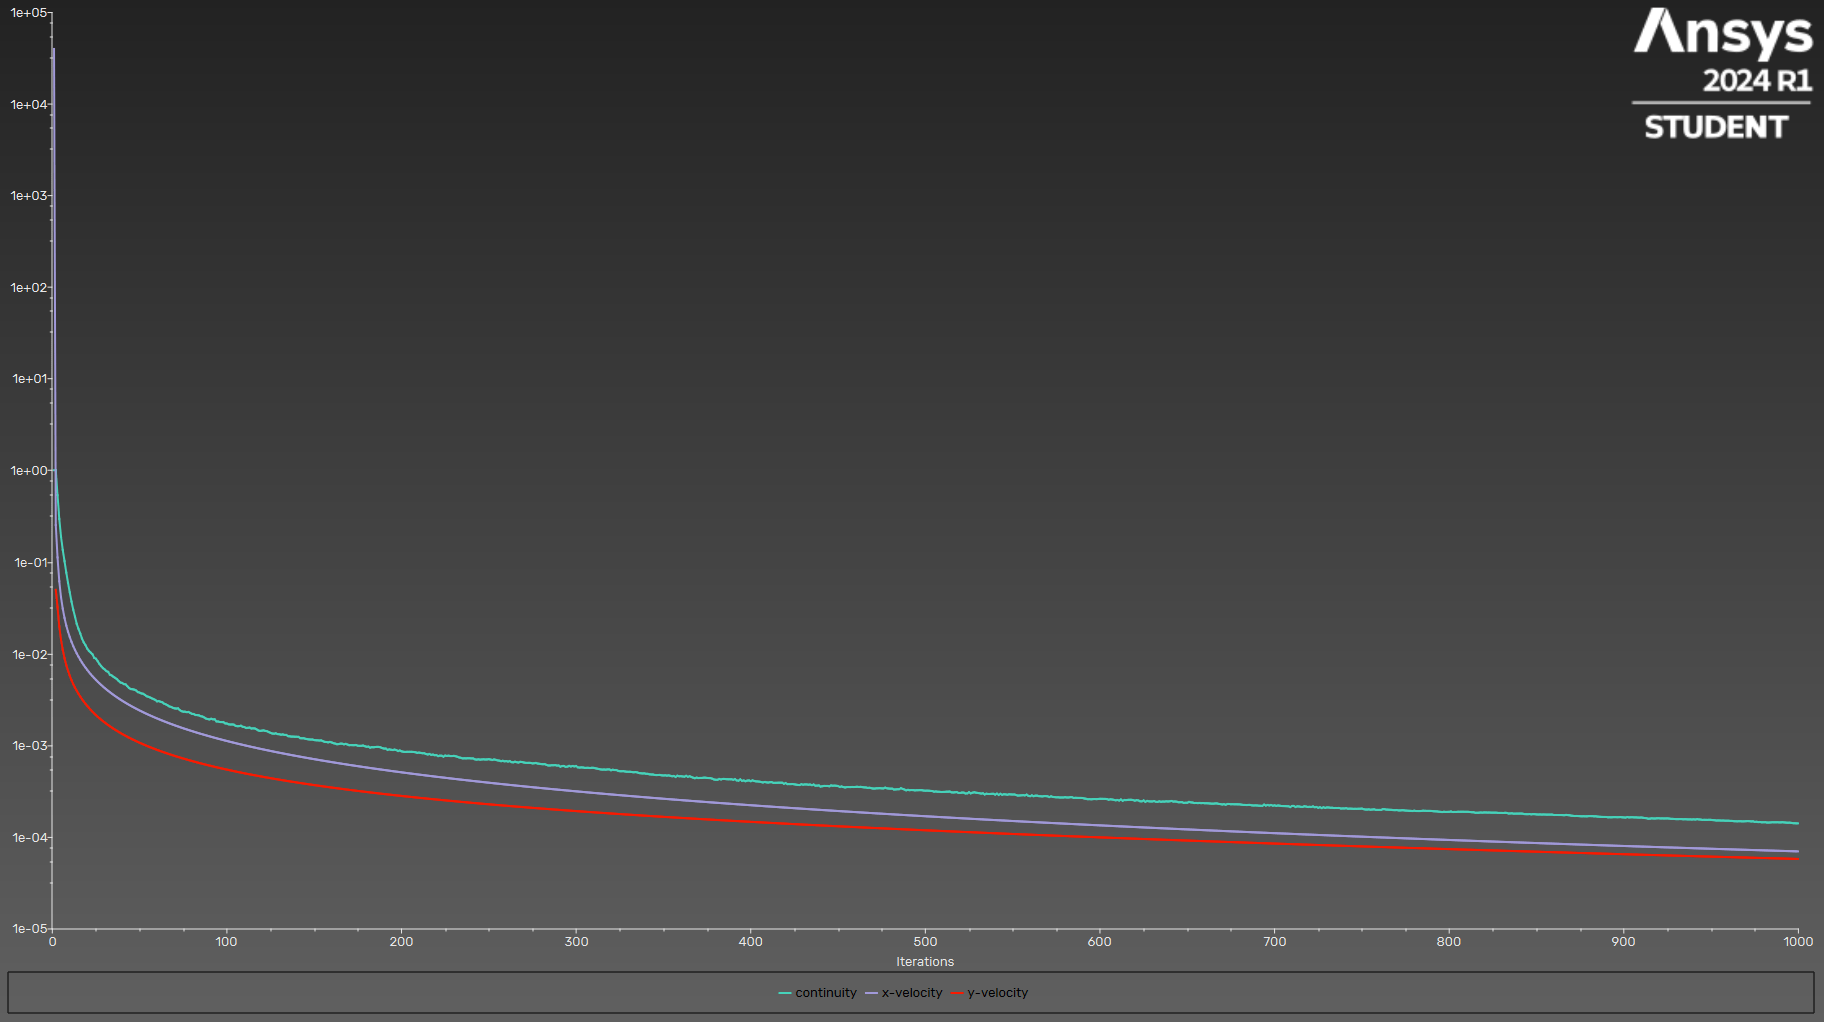
\includegraphics[width=\linewidth]{12.nal_slike/ansys/Re100-min.png}
        \caption{konvergenca residualov}
    \end{subfigure}
    \caption{$Re=100$}
\end{figure}

\begin{figure}[H]
    \centering
    \begin{subfigure}{0.49\textwidth}
        \centering
        \includegraphics[width=\linewidth]{12.nal_slike/ansys/Re8000_v-min.png}
        \caption{hitrostno polje}
    \end{subfigure}
    \begin{subfigure}{0.49\textwidth}
        \centering
        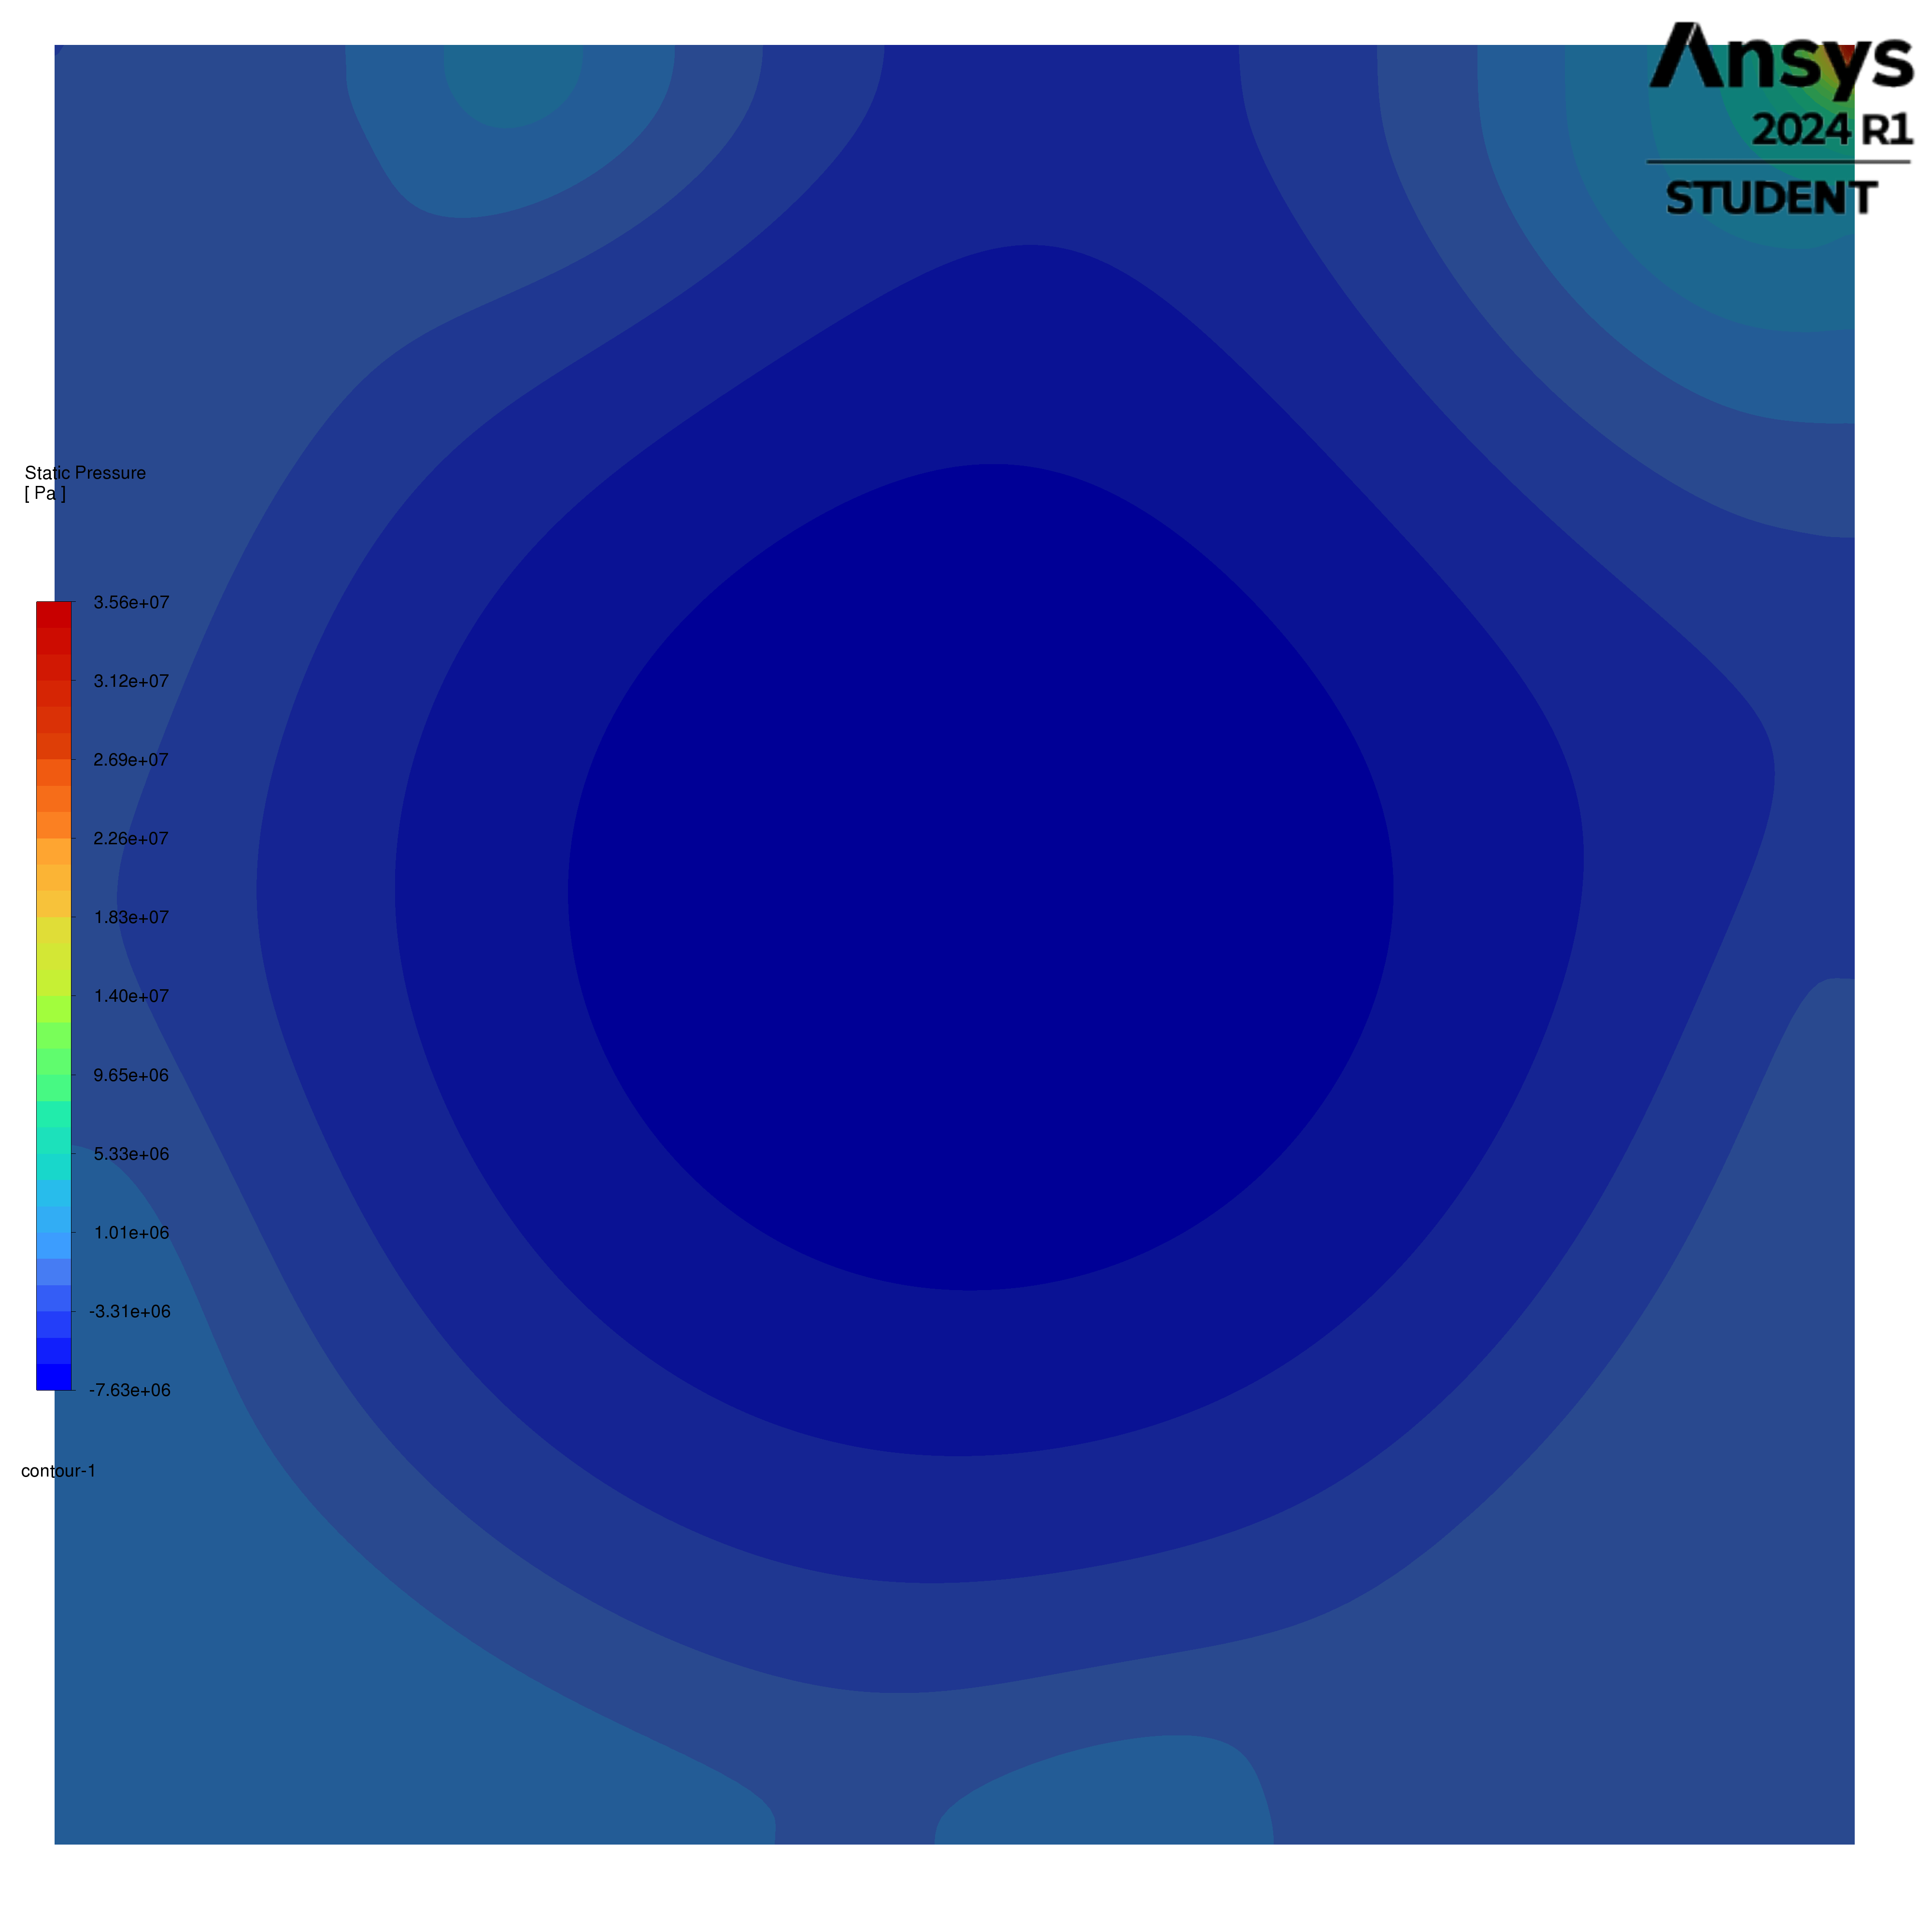
\includegraphics[width=\linewidth]{12.nal_slike/ansys/Re8000_p-min.png}
        \caption{tlačno polje}
    \end{subfigure}
    \caption{$Re=8000$}
\end{figure}